%! Author = crist
%! Date = 25/10/2026

\spacing{1.3}
%----------------------------------------------------------------------------------------
%	UNIDAD 1: EL TRABAJO CIENTÍFICO (4.º ESO)
%   Figuras: images/UD1/*.pdf (fuente HTML en images/UD1/html, SVG en images/UD1/svg)
%   Gráficas con pgfplots: estilo «grafica», que se define también aquí (la UD1 va antes que la UD7).
%----------------------------------------------------------------------------------------
\providecommand{\sen}{\operatorname{sen}}
\providecommand{\tg}{\operatorname{tg}}
\pgfplotsset{grafica/.style={
    width=7.5cm, height=5.2cm, axis lines=left, grid=both,
    grid style={line width=.1pt, draw=gray!20}, major grid style={line width=.3pt, draw=gray!40},
    label style={font=\small}, tick label style={font=\footnotesize},
    /pgf/number format/use comma,
    every axis plot/.append style={line width=1.4pt, color=red!75!black, mark=*, mark size=1.6pt}}}

% Mapa conceptual del tema (fuente en images/mapas_conceptuales/html/temas.js)
\begin{figure}[H]
    \centering
    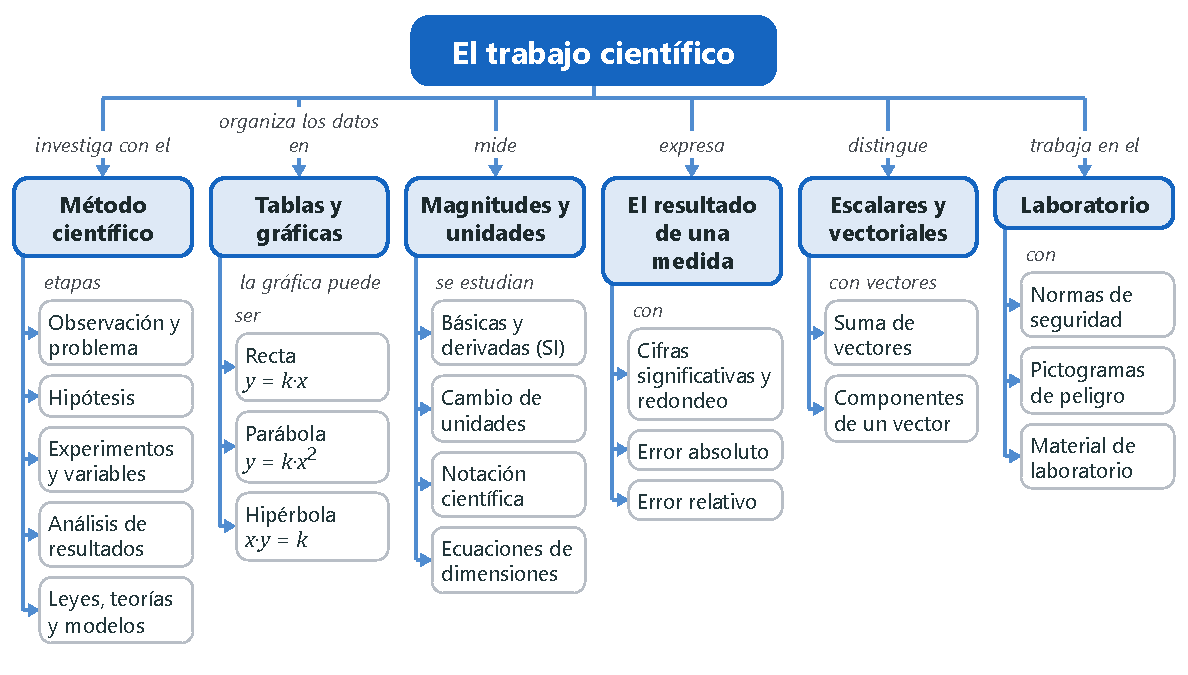
\includegraphics[width=\textwidth]{images/mapas_conceptuales/mapa_UD1}
\end{figure}

%========================================================================================
%\section*{Para empezar: Dorothy Hodgkin, bioquímica y cristalógrafa}
%\addcontentsline{toc}{section}{Para empezar: Dorothy Hodgkin, bioquímica y cristalógrafa}
%========================================================================================
%
%\textbf{Dorothy Hodgkin} (1910-1994) entró en la Universidad de Oxford en 1928, cuando la admisión de mujeres todavía estaba limitada. Se especializó en \textbf{cristalografía de rayos X}, una técnica entonces muy novedosa que permite averiguar la estructura de las moléculas, pero que exigía hacer a mano cálculos matemáticos larguísimos.
%
%En 1934 sorprendió con su trabajo sobre la estructura del colesterol, y se convirtió en la científica de referencia para «cartografiar» moléculas. Después se propuso averiguar la estructura de un antibiótico muy importante, la \textbf{penicilina}, descubierta por Alexander Fleming en 1928: los químicos necesitaban conocerla para poder fabricarla en el laboratorio. En 1945, tras cuatro años de trabajo y de crear nuevas técnicas de investigación, lo consiguió, y con ello contribuyó a salvar millones de vidas. Además, ideó un programa informático para cartografiar moléculas más deprisa, con el que determinó también las estructuras de la vitamina B\textsubscript{12} y de la insulina. Por todos sus logros recibió el Premio Nobel de Química en 1964.
%
%Su historia tiene que ver con el \textbf{ODS 4} (\emph{Educación de calidad}), que busca una educación inclusiva y equitativa y evitar la brecha de género en las carreras científicas y técnicas, y con el \textbf{ODS 3} (\emph{Salud y bienestar}), al que contribuyó con sus descubrimientos.
%
%En esta unidad aprenderemos cómo trabajan los científicos: en qué consiste el método científico, cómo se organizan y representan los datos, qué son las magnitudes y sus unidades, cómo se expresa el resultado de una medida, qué diferencia hay entre magnitudes escalares y vectoriales y qué normas de seguridad hay que seguir en el laboratorio.
%
%\begin{exercise}
%    ¿Qué tuvo de especial el ingreso de Dorothy Hodgkin en la Universidad de Oxford? ¿En qué especialidad destacó?
%    \begin{solu}
%        Entró en 1928, cuando todavía estaba \textcolor{red}{limitada la admisión de mujeres} en la universidad. Destacó en la \textcolor{red}{cristalografía de rayos X}.
%    \end{solu}
%\end{exercise}
%
%\begin{exercise}
%    ¿Qué herramienta creó para trabajar más deprisa? ¿Qué moléculas cartografió?
%    \begin{solu}
%        Un \textcolor{red}{programa informático} para cartografiar estructuras moleculares. Determinó las estructuras del \textcolor{red}{colesterol, la penicilina, la vitamina B\textsubscript{12} y la insulina}.
%    \end{solu}
%\end{exercise}
%
%\begin{exercise}
%    ¿Quién descubrió la penicilina? ¿Por qué era tan importante conocer la estructura de moléculas como la penicilina o la insulina?
%    \begin{solu}
%        \textcolor{red}{Alexander Fleming}, en 1928. Conocer su estructura permitía \textcolor{red}{fabricarlas en el laboratorio} (sintetizarlas) en grandes cantidades.
%    \end{solu}
%\end{exercise}
%
%\begin{exercise}
%    ¿Han contribuido sus descubrimientos a salvar vidas? ¿Qué relación tienen con los ODS 3 y 4?
%    \begin{solu}
%        \textcolor{red}{Sí}: la fabricación de penicilina e insulina ha permitido curar infecciones y tratar la diabetes a millones de personas, lo que contribuye a una vida sana (ODS 3). Su carrera muestra la importancia de que mujeres y hombres tengan el mismo acceso a la educación científica (ODS 4).
%    \end{solu}
%\end{exercise}

%========================================================================================
\section{¿En qué consiste el método científico?}
%========================================================================================

La \textbf{actividad científica} consiste en descubrir las leyes que rigen la naturaleza. Para ello se sigue un conjunto de etapas comunes a toda investigación, que llamamos \textbf{método científico} (figura~\ref{fig:metodo_cientifico}).

\begin{figure}[H]
    \centering
    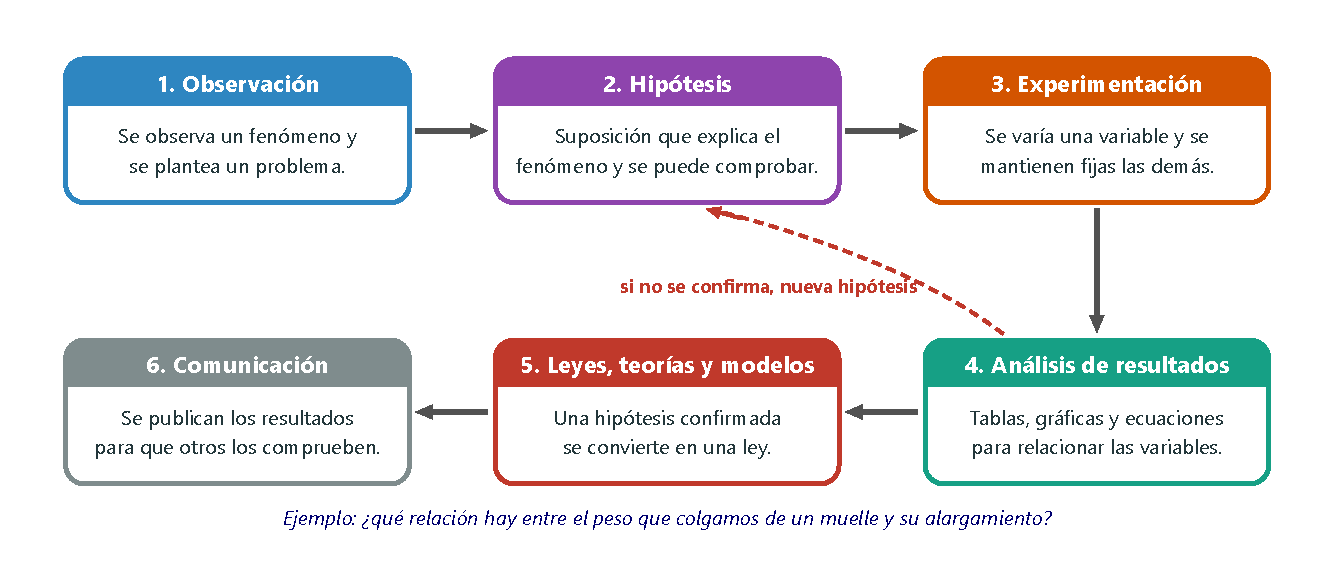
\includegraphics[width=\textwidth]{images/UD1/metodo_cientifico}
    \caption{Etapas del método científico.}
    \label{fig:metodo_cientifico}
\end{figure}

\subsection{Observación y planteamiento del problema}

Se observa con cuidado uno o más hechos o fenómenos con la intención de interpretarlos, lo que lleva a plantear preguntas. Por ejemplo, si colgamos una masa del extremo de un muelle, vemos que el muelle se alarga, y nos preguntamos: \emph{¿qué relación hay entre el peso que colgamos del muelle y el alargamiento que se produce?}

\subsection{Planteamiento de hipótesis}

\begin{definition}[Hipótesis científica]
    Una \textbf{hipótesis} es una suposición que intenta explicar un fenómeno. Para ser válida debe:
    \begin{itemize}
        \item Referirse a una situación real.
        \item Formularse de la forma más precisa posible, mediante variables concretas.
        \item Poder comprobarse experimentalmente, directamente o a través de sus consecuencias.
    \end{itemize}
\end{definition}

En el ejemplo, la hipótesis podría ser: \emph{el alargamiento del muelle es proporcional a la fuerza que se ejerce sobre él}.

\subsection{La experimentación}

Para saber si la hipótesis es cierta hay que comprobarla con hechos experimentales.

\begin{definition}[Experimentación y variables]
    La \textbf{experimentación} es la observación de un fenómeno en condiciones controladas.
    \begin{itemize}
        \item La \textbf{variable independiente} es la que el investigador va modificando.
        \item La \textbf{variable dependiente} es la que cambia como consecuencia y se mide para cada valor de la independiente.
        \item Las \textbf{variables controladas} son todas las demás, que deben mantenerse constantes.
    \end{itemize}
\end{definition}

Para comprobar nuestra hipótesis colgamos pesos diferentes del muelle y medimos los alargamientos (figura~\ref{fig:muelle_experimento}). El alargamiento es la longitud del muelle estirado, \(l\), menos su longitud natural, \(l_0\). La variable independiente es el peso que colgamos, y la dependiente, el alargamiento, \(l - l_0\).

\begin{figure}[H]
    \centering
    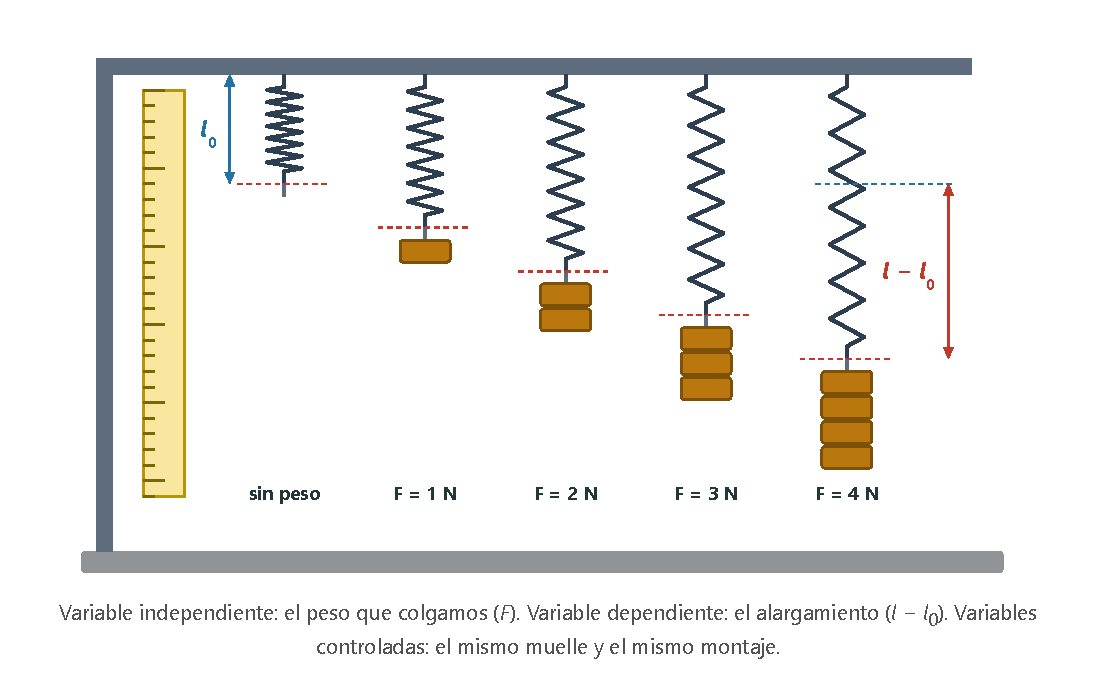
\includegraphics[width=0.85\textwidth]{images/UD1/muelle_experimento}
    \caption{Alargamiento de un muelle al colgar distintos pesos.}
    \label{fig:muelle_experimento}
\end{figure}

\subsection{Análisis de los resultados}

Los datos obtenidos se analizan para encontrar la relación entre las variables. Para ello se usan tablas, gráficas y otras herramientas matemáticas:

\begin{center}
    % --- tabla antigua ---
    % \begin{tblr}{colspec={lccccc}, hlines, vlines, row{1}={bg=ocre!85, fg=white, font=\bfseries}, column{1}={bg=ocre!85, fg=white, font=\bfseries}}
        % Fuerza, \(F\) (N) & \num{1.0} & \num{1.5} & \num{2.0} & \num{3.0} & \num{4.0} \\
        % Alargamiento, \(l - l_0\) (m) & \num{1.0e-2} & \num{1.5e-2} & \num{2.0e-2} & \num{3.0e-2} & \num{4.0e-2} \\
        % \(F/(l - l_0)\) (\unit{\newton\per\m}) & 100 & 100 & 100 & 100 & 100 \\
    % \end{tblr}
    % --- tabla nueva ---
    \begin{tabular}{@{}lccccc@{}}
        \toprule
        \textbf{Fuerza, \(F\) (N)} & \textbf{\num{1.0}} & \textbf{\num{1.5}} & \textbf{\num{2.0}} & \textbf{\num{3.0}} & \textbf{\num{4.0}} \\
        \midrule
        \textbf{Alargamiento, \(l - l_0\) (m)} & \num{1.0e-2} & \num{1.5e-2} & \num{2.0e-2} & \num{3.0e-2} & \num{4.0e-2} \\[3pt]
        \textbf{\(F/(l - l_0)\) (\unit{\newton\per\m})} & 100 & 100 & 100 & 100 & 100 \\
        \bottomrule
    \end{tabular}
\end{center}

\begin{center}
    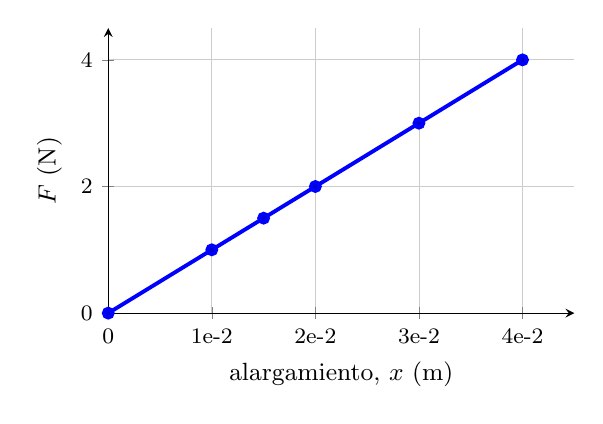
\begin{tikzpicture}
        \begin{axis}[grafica, xlabel={alargamiento, \(x\) (m)}, ylabel={\(F\) (N)}, xmin=0, xmax=0.045, ymin=0, ymax=4.5, scaled x ticks=false, xtick={0,0.01,0.02,0.03,0.04}, xticklabels={0, \num{1e-2}, \num{2e-2}, \num{3e-2}, \num{4e-2}}]
            \addplot coordinates {(0,0) (0.01,1) (0.015,1.5) (0.02,2) (0.03,3) (0.04,4)};
        \end{axis}
    \end{tikzpicture}
\end{center}

El cociente entre la fuerza y el alargamiento es constante y la gráfica es una recta que pasa por el origen: las dos magnitudes son \textbf{directamente proporcionales} y la hipótesis queda confirmada.

\subsection{Elaboración de leyes, teorías y modelos científicos}

Una vez analizados los resultados, se puede establecer una relación matemática entre los hechos observados.

\begin{definition}[Ley, teoría y modelo]
    Los resultados de la investigación científica se organizan en leyes, teorías y modelos:
    \begin{itemize}
        \item Una \textbf{ley científica} es una hipótesis confirmada. En el ejemplo, la relación entre el alargamiento del muelle, \(x\), y la fuerza aplicada, \(F\), es la \textbf{ley de Hooke}: \(F = k \cdot x\).
        \item Una \textbf{teoría científica} es un conjunto de leyes que explica las regularidades descritas por ellas.
        \item Un \textbf{modelo científico} es una representación mental simplificada que se usa para explicar algunos fenómenos. Por ejemplo, los modelos atómicos de Thomson, Rutherford y Bohr.
    \end{itemize}
\end{definition}

Por último, los resultados se \textbf{comunican} (en revistas científicas, congresos\ldots) para que otros investigadores puedan comprobarlos, criticarlos y ampliarlos.

\subsection{¿Qué diferencia hay entre causalidad y correlación?}

\begin{itemize}
    \item La \textbf{causalidad} es la relación entre una causa y su efecto. Por ejemplo, al aumentar la presión sobre un gas encerrado en un recipiente con un émbolo móvil (causa), su volumen disminuye (efecto).
    \item La \textbf{correlación} solo indica que dos variables cambian a la vez, sin que una sea necesariamente la causa de la otra. Por ejemplo, si dejamos caer desde la misma altura una bolita metálica y una hoja de papel de la misma masa, la bolita llega antes. Pero eso no significa que el tiempo de caída dependa de la masa (las dos tienen la misma): influye otro factor, la superficie de los cuerpos, que determina el rozamiento con el aire.
\end{itemize}

\subsection*{Actividades de consolidación: el método científico}

\begin{exercise}
    Todo lo que sucede en el universo se puede organizar y explicar con unas pocas leyes.
    \begin{enumerate}[label=\alph*)]
        \item Enuncia algunas leyes que conozcas.
        \item Además de la elaboración de leyes, teorías y modelos, ¿qué otras etapas tiene el método científico?
        \item Mariano Barbacid, María Blasco, Montserrat Calleja, Avelino Corma, Francis Mojica, Margarita Salas o Rafael Yuste destacan por sus investigaciones. Elige dos e investiga sus aportaciones a la ciencia.
        \item ¿Qué hipótesis se pueden plantear para responder a esta pregunta: ¿cómo afecta la temperatura a la solubilidad del azúcar en agua?
    \end{enumerate}
    \begin{solu}
        a) Respuesta abierta: las \textcolor{red}{leyes de Newton}, la ley de \textcolor{red}{gravitación universal}, la ley de \textcolor{red}{Hooke}, las leyes de los gases (\textcolor{red}{Boyle, Gay-Lussac}), la ley de conservación de la masa\ldots
        b) \textcolor{red}{Observación} y planteamiento del problema, \textcolor{red}{hipótesis}, \textcolor{red}{experimentación}, \textcolor{red}{análisis} de resultados y \textcolor{red}{comunicación}.
        c) Respuesta libre. Por ejemplo, Margarita Salas descubrió cómo se copia el ADN de un virus (la ADN polimerasa del fago \(\phi\)29), base de una técnica muy usada para amplificar ADN; Francis Mojica descubrió las secuencias CRISPR, que han dado lugar a una herramienta de edición genética.
        d) Por ejemplo: «la solubilidad del azúcar en agua \textcolor{red}{aumenta} al aumentar la temperatura», o bien «\textcolor{red}{disminuye}» o «\textcolor{red}{no cambia}». Para comprobarla, se mide cuánto azúcar se disuelve en la misma cantidad de agua a distintas temperaturas.
    \end{solu}
\end{exercise}

\begin{exercise}
    Para averiguar si el período de un péndulo (el tiempo que tarda en ir y volver) depende de la longitud del hilo, se mide con dos longitudes, \qty{0.5}{\m} y \qty{1.0}{\m}, manteniendo la misma masa. En tres medidas con cada péndulo se obtiene siempre \qty{1.42}{\s} para el de \qty{0.5}{\m} y \qty{2.00}{\s} para el de \qty{1.0}{\m}.
    \begin{enumerate}[label=\alph*)]
        \item Identifica la variable independiente, la dependiente y la controlada.
        \item ¿Varía el período al variar la longitud? ¿Crees que hay una relación de causalidad?
        \item Quieres comprobar si el período depende de la masa. ¿Cuál es tu hipótesis? ¿Cómo la comprobarías?
        \item Un compañero dice que, cerca del ecuador, los péndulos oscilan más despacio que en países del norte, y que se debe a la temperatura. Busca información y respóndele de forma científica.
    \end{enumerate}
    \begin{solu}
        a) Independiente: la \textcolor{red}{longitud} del hilo. Dependiente: el \textcolor{red}{período}. Controlada: la \textcolor{red}{masa} (y la amplitud de las oscilaciones).
        b) \textcolor{red}{Sí}: al aumentar la longitud aumenta el período. Hay \textcolor{red}{causalidad}, porque solo se ha cambiado la longitud y las demás variables se han mantenido constantes.
        c) Hipótesis: «el período \textcolor{red}{no depende} de la masa». Se comprueba midiendo el período de péndulos de la \textcolor{red}{misma longitud} con \textcolor{red}{masas distintas}.
        d) El período es algo mayor cerca del ecuador, pero no por la temperatura, sino porque allí la \textcolor{red}{gravedad es algo menor} (por la rotación de la Tierra y porque el ecuador está más lejos del centro de la Tierra): cuanto menor es \(g\), mayor es el período (\(T = 2\pi\sqrt{L/g}\)).
    \end{solu}
\end{exercise}

\begin{exercise}
    Explica las diferencias entre variable dependiente, independiente y controlada.
    \begin{solu}
        La \textcolor{red}{independiente} es la que modifica el investigador; la \textcolor{red}{dependiente} es la que se mide, porque cambia como consecuencia de la anterior; las \textcolor{red}{controladas} son las demás, que se mantienen constantes durante el experimento.
    \end{solu}
\end{exercise}

\begin{exercise}
    A lo largo del siglo \textsc{xx}, científicos de distintos países investigaron la radiactividad y algunos participaron en proyectos de armas nucleares. Busca información sobre algunos de ellos y debatid en clase la responsabilidad de los científicos.
    \begin{solu}
        Respuesta libre. Por ejemplo: Henri Becquerel, Marie y Pierre Curie (descubrimiento de la radiactividad), Ernest Rutherford, Lise Meitner y Otto Hahn (fisión nuclear), Enrico Fermi, Robert Oppenheimer (Proyecto Manhattan) o Joseph Rotblat, que abandonó el proyecto y luchó por el desarme nuclear (Nobel de la Paz en 1995).
    \end{solu}
\end{exercise}

%========================================================================================
\section[Tablas de datos y gráficas]{¿Qué información aportan las tablas de datos y las representaciones gráficas?}
%========================================================================================

Una \textbf{tabla de datos} está formada por filas y columnas: cada columna (o fila) corresponde a una variable y cada medida ocupa una casilla. Con la tabla elaboramos una \textbf{representación gráfica}, que muestra la relación entre las variables. Normalmente, la \textbf{variable independiente} se sitúa en el eje horizontal o de abscisas (eje X), y la \textbf{variable dependiente}, en el eje vertical o de ordenadas (eje Y). La forma de la línea indica qué relación hay entre ellas.

\subsection{Si la gráfica es una línea recta}

Una recta que pasa por el origen indica que las variables son \textbf{directamente proporcionales}: \(y = a \cdot x\), donde \(a\) es la pendiente. Si la recta no pasa por el origen, la ecuación es \(y = a \cdot x + b\), donde \(b\) es la ordenada en el origen.

A partir de una gráfica podemos predecir valores entre los medidos (\textbf{interpolar}) o fuera de ellos (\textbf{extrapolar}).

\subsection{Si la gráfica es una parábola}

Una \textbf{parábola} que pasa por el origen indica que la variable dependiente es proporcional al \textbf{cuadrado} de la independiente: \(y = a \cdot x^2\) (o \(y = a \cdot x^2 + b\) si no pasa por el origen). Por ejemplo, la distancia que recorre un cuerpo que parte del reposo con aceleración constante.

\subsection{Si la gráfica es una hipérbola}

Una \textbf{hipérbola} indica que las variables son \textbf{inversamente proporcionales}: \(y = k/x\), es decir, su producto es constante. Por ejemplo, la presión y el volumen de un gas a temperatura constante (ley de Boyle): \(p \cdot V = k\).

\begin{center}
    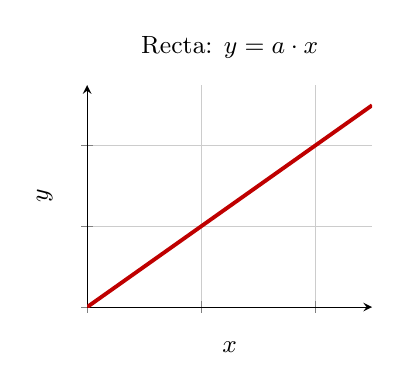
\begin{tikzpicture}
        \begin{axis}[grafica, width=5.2cm, height=4.4cm, xmin=0, xmax=5, ymin=0, ymax=5.5, xticklabels={}, yticklabels={}, xlabel={\(x\)}, ylabel={\(y\)}, title={\small Recta: \(y = a \cdot x\)}]
            \addplot[mark=none, domain=0:5, line width=1.4pt, color=red!75!black] {x};
        \end{axis}
    \end{tikzpicture}
    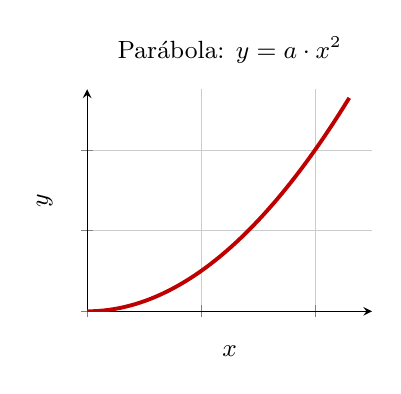
\begin{tikzpicture}
        \begin{axis}[grafica, width=5.2cm, height=4.4cm, xmin=0, xmax=5, ymin=0, ymax=5.5, xticklabels={}, yticklabels={}, xlabel={\(x\)}, ylabel={\(y\)}, title={\small Parábola: \(y = a \cdot x^2\)}]
            \addplot[mark=none, domain=0:4.6, samples=50, line width=1.4pt, color=red!75!black] {x^2/4};
        \end{axis}
    \end{tikzpicture}
    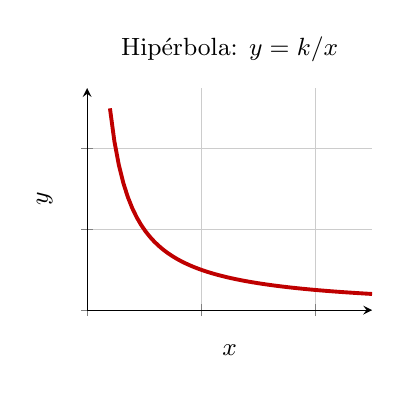
\begin{tikzpicture}
        \begin{axis}[grafica, width=5.2cm, height=4.4cm, xmin=0, xmax=5, ymin=0, ymax=5.5, xticklabels={}, yticklabels={}, xlabel={\(x\)}, ylabel={\(y\)}, title={\small Hipérbola: \(y = k/x\)}]
            \addplot[mark=none, domain=0.4:5, samples=60, line width=1.4pt, color=red!75!black] {2/x};
        \end{axis}
    \end{tikzpicture}
\end{center}

\begin{example}
    Un entrenador cronometra a un atleta que corre en línea recta:
    \begin{center}
        % --- tabla antigua ---
        % \begin{tblr}{colspec={lccccc}, hlines, vlines, column{1}={bg=ocre!85, fg=white, font=\bfseries}}
            % Espacio, \(s\) (m) & 0 & 16 & 32 & 64 & 100 \\
            % Tiempo, \(t\) (s) & 0 & 4 & 8 & 16 & 25 \\
        % \end{tblr}
        % --- tabla nueva ---
        \begin{tabular}{@{}lccccc@{}}
            \toprule
            \textbf{Espacio, \(s\) (m)} & 0 & 16 & 32 & 64 & 100 \\[3pt]
            \textbf{Tiempo, \(t\) (s)} & 0 & 4 & 8 & 16 & 25 \\
            \bottomrule
        \end{tabular}
    \end{center}
    \begin{enumerate}[label=\alph*)]
        \item Representa el espacio recorrido en función del tiempo y escribe la ecuación que los relaciona.
        \item ¿Qué espacio habrá recorrido a los \qty{30}{\s}? ¿Cuánto tarda en recorrer los primeros \qty{12}{\m}?
    \end{enumerate}

    \begin{center}
        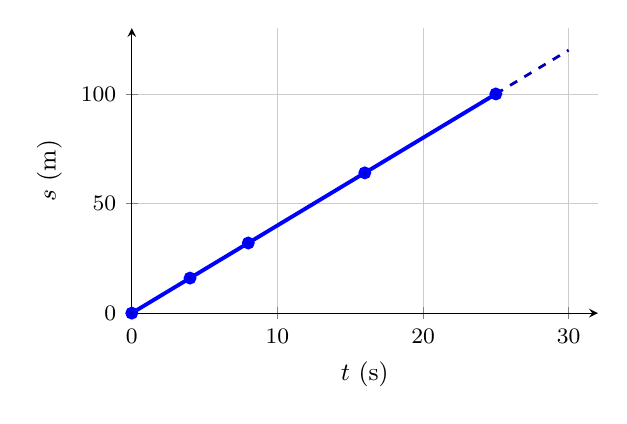
\begin{tikzpicture}
            \begin{axis}[grafica, xlabel={\(t\) (s)}, ylabel={\(s\) (m)}, xmin=0, xmax=32, ymin=0, ymax=130]
                \addplot coordinates {(0,0) (4,16) (8,32) (16,64) (25,100)};
                \addplot[mark=none, dashed, line width=1pt, color=blue!70!black] coordinates {(25,100) (30,120)};
            \end{axis}
        \end{tikzpicture}
    \end{center}

    a) La gráfica es una recta que pasa por el origen: \(s\) y \(t\) son directamente proporcionales. La pendiente es \(\dfrac{16}{4} = 4\), así que \textcolor{red}{\(s = 4 \cdot t\)} (con \(s\) en metros y \(t\) en segundos).

    b) Extrapolando: \(s = 4 \cdot 30 = \textcolor{red}{\qty{120}{\m}}\). Interpolando: \(12 = 4 \cdot t \Rightarrow t = \textcolor{red}{\qty{3}{\s}}\).
\end{example}

\begin{exercise}
    Se han medido las posiciones de un móvil a medida que transcurre el tiempo:
    \begin{center}
        % --- tabla antigua ---
        % \begin{tblr}{colspec={lcccccc}, hlines, vlines, column{1}={bg=ocre!85, fg=white, font=\bfseries}}
            % Posición, \(x\) (m) & 4 & 6 & 8 & 10 & 12 & 14 \\
            % Tiempo, \(t\) (s) & 0 & 1 & 2 & 3 & 4 & 5 \\
        % \end{tblr}
        % --- tabla nueva ---
        \begin{tabular}{@{}lcccccc@{}}
            \toprule
            \textbf{Posición, \(x\) (m)} & 4 & 6 & 8 & 10 & 12 & 14 \\[3pt]
            \textbf{Tiempo, \(t\) (s)} & 0 & 1 & 2 & 3 & 4 & 5 \\
            \bottomrule
        \end{tabular}
    \end{center}
    a) ¿En qué ejes situarías cada variable? b) Dibuja la gráfica posición-tiempo y escribe su ecuación.
    \begin{solu}
        a) El tiempo (variable independiente) en el \textcolor{red}{eje X}, y la posición (dependiente) en el \textcolor{red}{eje Y}.
        b) Es una \textcolor{red}{recta que no pasa por el origen}: pendiente \(\dfrac{2}{1} = 2\) y ordenada en el origen 4, así que \textcolor{red}{\(x = 4 + 2 \cdot t\)}.
        \begin{center}
            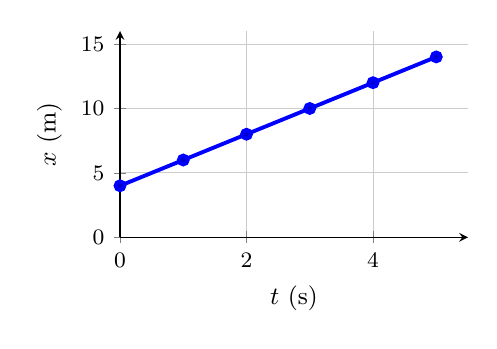
\begin{tikzpicture}
                \begin{axis}[grafica, width=6cm, height=4.2cm, xlabel={\(t\) (s)}, ylabel={\(x\) (m)}, xmin=0, xmax=5.5, ymin=0, ymax=16]
                    \addplot coordinates {(0,4) (1,6) (2,8) (3,10) (4,12) (5,14)};
                \end{axis}
            \end{tikzpicture}
        \end{center}
    \end{solu}
\end{exercise}

\subsection*{Actividades de consolidación: tablas de datos y gráficas}

\begin{exercise}
    En tres experimentos, las relaciones entre las variables son: a) \(y = 3x\); b) \(y = 10/x\); c) \(y = 5x^2\). ¿Qué forma tiene la gráfica de cada una? ¿Qué tipo de relación indica?
    \begin{solu}
        a) \textcolor{red}{Recta} que pasa por el origen: proporcionalidad directa.
        b) \textcolor{red}{Hipérbola}: proporcionalidad inversa.
        c) \textcolor{red}{Parábola}: \(y\) es proporcional al cuadrado de \(x\).
    \end{solu}
\end{exercise}

\begin{exercise}
    Estos son los valores de la velocidad de un móvil:
    \begin{center}
        % --- tabla antigua ---
        % \begin{tblr}{colspec={lcccc}, hlines, vlines, column{1}={bg=ocre!85, fg=white, font=\bfseries}}
            % Velocidad (m/s) & 0 & 3 & 6 & 9 \\
            % Tiempo (s) & 0 & 1 & 2 & 3 \\
        % \end{tblr}
        % --- tabla nueva ---
        \begin{tabular}{@{}lcccc@{}}
            \toprule
            \textbf{Velocidad (m/s)} & 0 & 3 & 6 & 9 \\[3pt]
            \textbf{Tiempo (s)} & 0 & 1 & 2 & 3 \\
            \bottomrule
        \end{tabular}
    \end{center}
    a) Dibuja la gráfica velocidad-tiempo. b) ¿Qué información proporciona? c) Escribe la ecuación que relaciona las variables. d) ¿En qué instantes la velocidad es \qty{4}{\m\per\s} y \qty{8}{\m\per\s}?
    \begin{solu}
        a) Una recta que pasa por el origen (tiempo en el eje X, velocidad en el eje Y).
        b) La velocidad y el tiempo son \textcolor{red}{directamente proporcionales}: la velocidad aumenta \qty{3}{\m\per\s} cada segundo.
        c) \textcolor{red}{\(v = 3 \cdot t\)}.
        d) \(4 = 3t \Rightarrow t = \textcolor{red}{\qty{1.33}{\s}}\); \(8 = 3t \Rightarrow t = \textcolor{red}{\qty{2.67}{\s}}\).
    \end{solu}
\end{exercise}

\begin{exercise}
    En un experimento con un gas a temperatura constante se obtienen estos datos. Comprueba que la presión y el volumen son inversamente proporcionales y calcula el volumen cuando la presión es \qty{2.5}{\atm}.
    \begin{center}
        % --- tabla antigua ---
        % \begin{tblr}{colspec={lcccc}, hlines, vlines, column{1}={bg=ocre!85, fg=white, font=\bfseries}}
            % Volumen (L) & \num{4.0} & \num{3.2} & \num{2.5} & \num{2.0} \\
            % Presión (atm) & \num{1.00} & \num{1.25} & \num{1.60} & \num{2.00} \\
        % \end{tblr}
        % --- tabla nueva ---
        \begin{tabular}{@{}lcccc@{}}
            \toprule
            \textbf{Volumen (L)} & \num{4.0} & \num{3.2} & \num{2.5} & \num{2.0} \\[3pt]
            \textbf{Presión (atm)} & \num{1.00} & \num{1.25} & \num{1.60} & \num{2.00} \\
            \bottomrule
        \end{tabular}
    \end{center}
    \begin{solu}
        El producto \(p \cdot V\) vale siempre \(\num{4.0}~\unit{\atm\liter}\) (\(1 \cdot 4 = \num{1.25} \cdot \num{3.2} = \num{1.6} \cdot \num{2.5} = 2 \cdot 2 = 4\)): son \textcolor{red}{inversamente proporcionales} (la gráfica es una hipérbola).
        \(V = \dfrac{4}{\num{2.5}} = \textcolor{red}{\qty{1.6}{\liter}}\).
    \end{solu}
\end{exercise}

%========================================================================================
\section[Magnitudes básicas y derivadas]{¿Qué es una magnitud? Magnitudes básicas y derivadas}
%========================================================================================

\begin{definition}[Magnitud y unidad]
    Una \textbf{magnitud} es cualquier propiedad de los cuerpos que se puede medir. \textbf{Medir} una magnitud es compararla con otra de la misma naturaleza, llamada \textbf{unidad}, para saber cuántas veces la contiene.
\end{definition}

Las \textbf{magnitudes básicas} se definen por sí mismas, mientras que las \textbf{magnitudes derivadas} se obtienen a partir de operaciones matemáticas con las básicas.

\subsection{El Sistema Internacional de Unidades (SI)}

\begin{center}
    % --- tabla antigua ---
    % \begin{tblr}{colspec={lccc}, hlines, vlines, row{1}={bg=ocre!85, fg=white, font=\bfseries\small}, cells={font=\small}}
        % Magnitud básica & Símbolo & Unidad & Símbolo \\
        % Longitud & \(L\) & metro & \unit{\m} \\
        % Masa & \(m\) & kilogramo & \unit{\kg} \\
        % Tiempo & \(t\) & segundo & \unit{\s} \\
        % Temperatura & \(T\) & kelvin & \unit{\kelvin} \\
        % Intensidad de corriente & \(I\) & amperio & \unit{\ampere} \\
        % Intensidad luminosa & \(I_v\) & candela & \unit{\candela} \\
        % Cantidad de sustancia & \(n\) & mol & \unit{\mol} \\
    % \end{tblr}
    % --- tabla nueva ---
    {\small
    \begin{tabular}{@{}lccc@{}}
        \toprule
        \textbf{Magnitud básica} & \textbf{Símbolo} & \textbf{Unidad} & \textbf{Símbolo} \\
        \midrule
        Longitud & \(L\) & metro & \unit{\m} \\[3pt]
        Masa & \(m\) & kilogramo & \unit{\kg} \\[3pt]
        Tiempo & \(t\) & segundo & \unit{\s} \\[3pt]
        Temperatura & \(T\) & kelvin & \unit{\kelvin} \\[3pt]
        Intensidad de corriente & \(I\) & amperio & \unit{\ampere} \\[3pt]
        Intensidad luminosa & \(I_v\) & candela & \unit{\candela} \\[3pt]
        Cantidad de sustancia & \(n\) & mol & \unit{\mol} \\
        \bottomrule
    \end{tabular}
    }
    \quad
    % --- tabla antigua ---
    % \begin{tblr}{colspec={lccc}, hlines, vlines, row{1}={bg=ocre!85, fg=white, font=\bfseries\small}, cells={font=\small}}
        % Magnitud derivada & Símbolo & Unidad SI & Otras \\
        % Superficie & \(S\) & \unit{\square\m} & -- \\
        % Volumen & \(V\) & \unit{\cubic\m} & L \\
        % Densidad & \(\rho\) & \unit{\kg\per\cubic\m} & g/mL \\
        % Velocidad & \(v\) & \unit{\m\per\s} & km/h \\
        % Aceleración & \(a\) & \unit{\m\per\square\s} & -- \\
        % Fuerza & \(F\) & N (newton) & -- \\
        % Presión & \(p\) & Pa (pascal) & atm, mmHg \\
        % Energía & \(E\) & J (julio) & eV \\
    % \end{tblr}
    % --- tabla nueva ---
    {\small
    \begin{tabular}{@{}lccc@{}}
        \toprule
        \textbf{Magnitud derivada} & \textbf{Símbolo} & \textbf{Unidad SI} & \textbf{Otras} \\
        \midrule
        Superficie & \(S\) & \unit{\square\m} & -- \\[3pt]
        Volumen & \(V\) & \unit{\cubic\m} & L \\[3pt]
        Densidad & \(\rho\) & \unit{\kg\per\cubic\m} & g/mL \\[3pt]
        Velocidad & \(v\) & \unit{\m\per\s} & km/h \\[3pt]
        Aceleración & \(a\) & \unit{\m\per\square\s} & -- \\[3pt]
        Fuerza & \(F\) & N (newton) & -- \\[3pt]
        Presión & \(p\) & Pa (pascal) & atm, mmHg \\[3pt]
        Energía & \(E\) & J (julio) & eV \\
        \bottomrule
    \end{tabular}
    }
\end{center}

Para expresar medidas muy grandes o muy pequeñas se usan los múltiplos y submúltiplos de las unidades, con estos prefijos:

\begin{center}
    % --- tabla antigua ---
    % \begin{tblr}{colspec={cccccc}, hlines, vlines, row{1}={bg=ocre!85, fg=white, font=\bfseries\small}, cells={font=\small}}
        % \num{e12} & \num{e9} & \num{e6} & \num{e3} & \num{e2} & \num{e1} \\
        % tera- (T) & giga- (G) & mega- (M) & kilo- (k) & hecto- (h) & deca- (da) \\
    % \end{tblr}
    % --- tabla nueva ---
    {\small
    \begin{tabular}{@{}cccccc@{}}
        \toprule
        \textbf{\num{e12}} & \textbf{\num{e9}} & \textbf{\num{e6}} & \textbf{\num{e3}} & \textbf{\num{e2}} & \textbf{\num{e1}} \\
        \midrule
        tera- (T) & giga- (G) & mega- (M) & kilo- (k) & hecto- (h) & deca- (da) \\
        \bottomrule
    \end{tabular}
    }
    \\[1ex]
    % --- tabla antigua ---
    % \begin{tblr}{colspec={cccccc}, hlines, vlines, row{1}={bg=ocre!85, fg=white, font=\bfseries\small}, cells={font=\small}}
        % \num{e-1} & \num{e-2} & \num{e-3} & \num{e-6} & \num{e-9} & \num{e-12} \\
        % deci- (d) & centi- (c) & mili- (m) & micro- (\(\mu\)) & nano- (n) & pico- (p) \\
    % \end{tblr}
    % --- tabla nueva ---
    {\small
    \begin{tabular}{@{}cccccc@{}}
        \toprule
        \textbf{\num{e-1}} & \textbf{\num{e-2}} & \textbf{\num{e-3}} & \textbf{\num{e-6}} & \textbf{\num{e-9}} & \textbf{\num{e-12}} \\
        \midrule
        deci- (d) & centi- (c) & mili- (m) & micro- (\(\mu\)) & nano- (n) & pico- (p) \\
        \bottomrule
    \end{tabular}
    }
\end{center}

\subsection{¿Cómo se transforman unas unidades en otras?}

Las medidas que no están en unidades del SI se transforman multiplicando por \textbf{factores de conversión}, fracciones que valen 1 (numerador y denominador expresan la misma cantidad):
\[ \qty{72}{\km\per\hour} = 72~\frac{\unit{\km}}{\unit{\hour}} \cdot \frac{\qty{e3}{\m}}{\qty{1}{\km}} \cdot \frac{\qty{1}{\hour}}{\qty{3600}{\s}} = \qty{20}{\m\per\s} \]
\[ \qty{11.34}{\gram\per\cubic\cm} = \num{11.34}~\frac{\unit{\gram}}{\unit{\cubic\cm}} \cdot \frac{\qty{1}{\kg}}{\qty{e3}{\gram}} \cdot \frac{\qty{e6}{\cubic\cm}}{\qty{1}{\cubic\m}} = \qty{11340}{\kg\per\cubic\m} \]

\subsection{¿Cómo se utiliza la notación científica?}

La \textbf{notación científica} consiste en escribir un número como un decimal con \textbf{una sola cifra entera} (distinta de cero) multiplicado por una \textbf{potencia de 10}, con exponente positivo o negativo. Para ello se desplaza la coma hasta que quede una sola cifra a su izquierda, y el número de lugares que se ha desplazado es el exponente:
\[ \qty{150000000000}{\m} = \qty{1.5e11}{\m} \qquad\qquad \qty{0.0000000002}{\m} = \qty{2e-10}{\m} \]
La distancia de la Tierra al Sol (\(1~\text{UA} = \qty{1.5e11}{\m}\)) se usa como unidad para las distancias del sistema solar, y el \textbf{año luz} (la distancia que recorre la luz en un año, unos \qty{9.46e15}{\m}), para las distancias entre estrellas y galaxias.

\begin{exercise}
    Transforma: a) a \unit{\m\per\s}: \qty{36}{\km\per\hour}, \qty{100}{\km\per\hour}, \qty{120}{\km\per\hour}; b) a \unit{\km\per\hour}: \qty{12}{\m\per\s}, \qty{340}{\m\per\s}, \qty{0.36}{\m\per\s}.
    \begin{solu}
        Para pasar de km/h a m/s se divide entre \num{3.6}, y al revés se multiplica.
        a) \textcolor{red}{\qty{10}{\m\per\s}}; \textcolor{red}{\qty{27.8}{\m\per\s}}; \textcolor{red}{\qty{33.3}{\m\per\s}}.
        b) \textcolor{red}{\qty{43.2}{\km\per\hour}}; \textcolor{red}{\qty{1224}{\km\per\hour}}; \textcolor{red}{\qty{1.3}{\km\per\hour}}.
    \end{solu}
\end{exercise}

\begin{exercise}
    Escribe en notación científica: a) \qty{0.00005}{\gram}; b) \qty{0.000052}{\gram}; c) \qty{2000000}{\m}; d) \qty{25000000}{\m}; e) \qty{3010000}{\s}; f) \qty{0.000205}{\ampere}.
    \begin{solu}
        a) \textcolor{red}{\qty{5e-5}{\gram}}; b) \textcolor{red}{\qty{5.2e-5}{\gram}}; c) \textcolor{red}{\qty{2e6}{\m}}; d) \textcolor{red}{\qty{2.5e7}{\m}}; e) \textcolor{red}{\qty{3.01e6}{\s}}; f) \textcolor{red}{\qty{2.05e-4}{\ampere}}.
    \end{solu}
\end{exercise}

\begin{exercise}
    Expresa en unidades del SI con notación científica: a) \qty{500}{\hecto\m}; b) \qty{3}{\deci\gram}; c) \qty{125}{\km}; d) \qty{250}{\gram}; e) \qty{25}{\mA}; f) \qty{1.25}{\cubic\dm}; g) \qty{9}{\us}; h) \qty{0.99}{\hecto\pascal}.
    \begin{solu}
        a) \textcolor{red}{\qty{5e4}{\m}}; b) \textcolor{red}{\qty{3e-4}{\kg}}; c) \textcolor{red}{\qty{1.25e5}{\m}}; d) \textcolor{red}{\qty{2.5e-1}{\kg}}; e) \textcolor{red}{\qty{2.5e-2}{\ampere}}; f) \textcolor{red}{\qty{1.25e-3}{\cubic\m}}; g) \textcolor{red}{\qty{9e-6}{\s}}; h) \textcolor{red}{\qty{99}{\pascal}} \(= \qty{9.9e1}{\pascal}\).
    \end{solu}
\end{exercise}

\begin{exercise}
    La densidad del argón es \qty{1.784}{\kg\per\cubic\m}. ¿Qué masa tiene \qty{1}{\cubic\cm} de argón?
    \begin{solu}
        \(\num{1.784}~\unit{\kg\per\cubic\m} = \num{1.784e-3}~\unit{\gram\per\cubic\cm}\); \(m = \rho \cdot V = \num{1.784e-3} \cdot 1 = \textcolor{red}{\qty{1.784e-3}{\gram}}\).
    \end{solu}
\end{exercise}

\begin{exercise}
    El récord de velocidad de un Fórmula 1, alcanzado en un entrenamiento en 2016, es de \qty{378}{\km\per\hour}. Exprésalo en \unit{\m\per\s}.
    \begin{solu}
        \(\dfrac{378}{\num{3.6}} = \textcolor{red}{\qty{105}{\m\per\s}}\).
    \end{solu}
\end{exercise}

\subsection*{Actividades de consolidación: magnitudes y unidades}

\begin{exercise}
    Clasifica en básicas o derivadas: densidad, longitud, volumen, masa, presión, temperatura, fuerza, trabajo, intensidad de corriente, superficie, energía, aceleración, cantidad de sustancia y velocidad.
    \begin{solu}
        Básicas: \textcolor{red}{longitud, masa, temperatura, intensidad de corriente y cantidad de sustancia}. Derivadas: \textcolor{red}{densidad, volumen, presión, fuerza, trabajo, superficie, energía, aceleración y velocidad}.
    \end{solu}
\end{exercise}

\begin{exercise}
    Escribe en notación científica y en unidades del SI:
    \begin{enumerate}[label=\alph*)]
        \item La distancia de la Tierra a la Luna: \qty{384400}{\km}.
        \item La distancia entre el átomo de hidrógeno y el de oxígeno en el agua: \qty{0.000000000097}{\m}.
        \item La distancia de Júpiter al Sol: \qty{778500000}{\km}.
        \item La masa de la Tierra: \qty{6000000000000000000000000}{\kg}.
        \item El tamaño de una bacteria: \qty{5}{\um}; el de un virus: \qty{24}{\nm}.
        \item El tiempo que tarda la luz del Sol en llegar a la Tierra: \qty{8}{\minute} \qty{20}{\s}.
    \end{enumerate}
    \begin{solu}
        a) \textcolor{red}{\qty{3.844e8}{\m}}; b) \textcolor{red}{\qty{9.7e-11}{\m}}; c) \textcolor{red}{\qty{7.785e11}{\m}}; d) \textcolor{red}{\qty{6e24}{\kg}}; e) \textcolor{red}{\qty{5e-6}{\m}}; \textcolor{red}{\qty{2.4e-8}{\m}}; f) \(8 \cdot 60 + 20 = \textcolor{red}{\qty{5.0e2}{\s}}\).
    \end{solu}
\end{exercise}

\begin{exercise}
    Expresa en notación científica: a) \qty{0.000008}{\ampere}; b) \qty{205000000}{\m}; c) \qty{0.00305}{\kg}; d) \qty{145000}{\s}.
    \begin{solu}
        a) \textcolor{red}{\qty{8e-6}{\ampere}}; b) \textcolor{red}{\qty{2.05e8}{\m}}; c) \textcolor{red}{\qty{3.05e-3}{\kg}}; d) \textcolor{red}{\qty{1.45e5}{\s}}.
    \end{solu}
\end{exercise}

\begin{exercise}
    La velocidad del sonido es \qty{1270}{\m\per\s} en el hidrógeno, \qty{927}{\m\per\s} en el helio, \qty{258}{\m\per\s} en el dióxido de carbono y \qty{340}{\m\per\s} en el aire. Exprésalas en \unit{\km\per\hour}.
    \begin{solu}
        Se multiplica por \num{3.6}: hidrógeno, \textcolor{red}{\qty{4572}{\km\per\hour}}; helio, \textcolor{red}{\qty{3337}{\km\per\hour}}; dióxido de carbono, \textcolor{red}{\qty{929}{\km\per\hour}}; aire, \textcolor{red}{\qty{1224}{\km\per\hour}}.
    \end{solu}
\end{exercise}

\begin{exercise}
    Expresa en unidades del SI con notación científica: a) \qty{300000}{\km\per\s}; b) \qty{2.5}{\hour}; c) \qty{10.5}{\gram\per\cubic\cm}. ¿Cuánto es la densidad media de la Tierra, \qty{5.51}{\gram\per\cubic\cm}, en unidades del SI?
    \begin{solu}
        a) \textcolor{red}{\qty{3e8}{\m\per\s}}; b) \(\num{2.5} \cdot 3600 = \textcolor{red}{\qty{9e3}{\s}}\); c) \textcolor{red}{\qty{1.05e4}{\kg\per\cubic\m}}. Tierra: \textcolor{red}{\qty{5510}{\kg\per\cubic\m}} \(= \qty{5.51e3}{\kg\per\cubic\m}\).
    \end{solu}
\end{exercise}

\begin{exercise}
    Un depósito cilíndrico tiene \qty{4}{\m} de altura y \qty{1}{\m} de radio. ¿Cuántos litros de agua contiene si el nivel está a \(1/3\) de la altura por debajo del borde superior?
    \begin{solu}
        La altura del agua es \(\frac{2}{3} \cdot 4 = \qty{2.67}{\m}\). \(V = \pi \cdot r^2 \cdot h = \pi \cdot 1^2 \cdot \num{2.67} = \qty{8.38}{\cubic\m} = \textcolor{red}{\qty{8378}{\liter}}\) (\(\approx \num{8.4e3}\) L).
    \end{solu}
\end{exercise}

\begin{exercise}
    La figura muestra el plano de una finca (cada cuadrado de la cuadrícula mide \(1 \times 1\)~\unit{\m}). Calcula su superficie dividiéndola en figuras sencillas.
    \begin{center}
        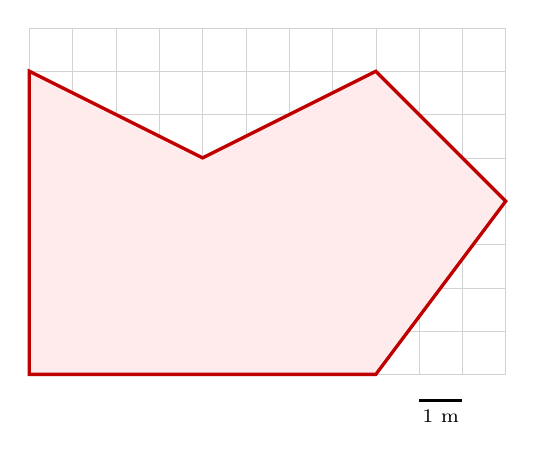
\begin{tikzpicture}[scale=0.55]
            \draw[step=1, gray!35, very thin] (0,0) grid (11,8);
            \draw[red!75!black, very thick, fill=red!8] (0,0) -- (8,0) -- (11,4) -- (8,7) -- (4,5) -- (0,7) -- cycle;
            \draw[thick] (9,-0.6) -- (10,-0.6); \node[below, font=\scriptsize] at (9.5,-0.6) {1 m};
        \end{tikzpicture}
    \end{center}
    \begin{solu}
        Partimos del rectángulo de \(8 \times 7\)~\unit{\m}: \(S_1 = 8 \cdot 7 = \qty{56}{\square\m}\).
        Le sumamos el triángulo de la derecha, de base 7 (el lado vertical \(x = 8\)) y altura 3: \(S_2 = \frac{1}{2} \cdot 7 \cdot 3 = \qty{10.5}{\square\m}\).
        Le restamos el triángulo de la muesca de arriba, de base 8 y altura 2: \(S_3 = \frac{1}{2} \cdot 8 \cdot 2 = \qty{8}{\square\m}\).
        \(S = 56 + \num{10.5} - 8 = \textcolor{red}{\qty{58.5}{\square\m}}\).
    \end{solu}
\end{exercise}

\begin{exercise}
    Indica la cantidad mayor de cada pareja: a) \qty{1600}{\gram} o \qty{1.5}{\kg}; b) \qty{1450}{\mm} o \qty{1.3}{\m}; c) \qty{320}{\s} o \qty{5}{\minute}; d) \qty{200}{\square\cm} o \qty{2}{\square\m}; e) \qty{0.000125}{\cubic\m} o \qty{125}{\cubic\m}.
    \begin{solu}
        a) \textcolor{red}{\qty{1600}{\gram}} (\qty{1.6}{\kg}); b) \textcolor{red}{\qty{1450}{\mm}} (\qty{1.45}{\m}); c) \textcolor{red}{\qty{320}{\s}} (\qty{5}{\minute} son \qty{300}{\s}); d) \textcolor{red}{\qty{2}{\square\m}}; e) \textcolor{red}{\qty{125}{\cubic\m}}.
    \end{solu}
\end{exercise}

\begin{exercise}
    Expresa en notación científica: a) \qty{60000000}{\m}; b) \qty{32000000}{\m}; c) \qty{9820000000}{\m}; d) \qty{570000}{\s}; e) \qty{0.005}{\s}; f) \qty{0.000075}{\kg}; g) \qty{0.00009}{\kg}; h) \qty{8000000000}{\kg}.
    \begin{solu}
        a) \textcolor{red}{\qty{6e7}{\m}}; b) \textcolor{red}{\qty{3.2e7}{\m}}; c) \textcolor{red}{\qty{9.82e9}{\m}}; d) \textcolor{red}{\qty{5.7e5}{\s}}; e) \textcolor{red}{\qty{5e-3}{\s}}; f) \textcolor{red}{\qty{7.5e-5}{\kg}}; g) \textcolor{red}{\qty{9e-5}{\kg}}; h) \textcolor{red}{\qty{8e9}{\kg}}.
    \end{solu}
\end{exercise}

%========================================================================================
\section{Ecuaciones de dimensiones}
%========================================================================================

Solo tiene sentido sumar o restar cantidades de la misma naturaleza: no podemos sumar una longitud y una temperatura. Para que una ecuación como \(A = B + C\) tenga sentido, \(A\), \(B\) y \(C\) deben tener las mismas \textbf{dimensiones}.

Las \textbf{dimensiones básicas} son las de las magnitudes básicas: longitud (L), masa (M), tiempo (T), intensidad de corriente (I), temperatura (\(\Theta\)), cantidad de sustancia (N) e intensidad luminosa (J). La \textbf{ecuación de dimensiones} de una magnitud expresa sus dimensiones en función de las básicas; se escribe el símbolo de la magnitud entre corchetes y se obtiene de su definición, prescindiendo de los números:
\[ [v] = \frac{[s]}{[t]} = \mathrm{L \cdot T^{-1}} \qquad [a] = \frac{[v]}{[t]} = \mathrm{L \cdot T^{-2}} \qquad [F] = [m] \cdot [a] = \mathrm{M \cdot L \cdot T^{-2}} \]

Las ecuaciones de dimensiones permiten comprobar si una ecuación física puede ser correcta: los dos miembros deben tener las mismas dimensiones (ecuación \textbf{homogénea}).

\begin{example}
    Comprueba que la ecuación de la fuerza centrípeta, \(F = \dfrac{m \cdot v^2}{r}\), es homogénea.

    Primer miembro: \([F] = \mathrm{M \cdot L \cdot T^{-2}}\). Segundo miembro: \(\dfrac{[m] \cdot [v]^2}{[r]} = \dfrac{\mathrm{M} \cdot (\mathrm{L \cdot T^{-1}})^2}{\mathrm{L}} = \mathrm{M \cdot L \cdot T^{-2}}\). Coinciden: \textcolor{red}{es homogénea}.
\end{example}

\begin{exercise}
    Escribe la ecuación de dimensiones del volumen y de la densidad.
    \begin{solu}
        \([V] = \textcolor{red}{\mathrm{L^3}}\); \([\rho] = \dfrac{[m]}{[V]} = \textcolor{red}{\mathrm{M \cdot L^{-3}}}\).
    \end{solu}
\end{exercise}

\begin{exercise}
    ¿Cuál de estas ecuaciones de dimensiones corresponde a la aceleración? a) \(\mathrm{L \cdot T^{-2}}\); b) \(\mathrm{L^{-2} \cdot T}\).
    \begin{solu}
        La \textcolor{red}{a)}: la aceleración es una velocidad (\(\mathrm{L \cdot T^{-1}}\)) dividida entre un tiempo.
    \end{solu}
\end{exercise}

\subsection*{Actividades de consolidación: ecuaciones de dimensiones}

\begin{exercise}
    ¿Qué es la ecuación de dimensiones de una magnitud? Pon un ejemplo.
    \begin{solu}
        Es la expresión de una magnitud en función de las \textcolor{red}{dimensiones básicas}. Por ejemplo, la velocidad es espacio entre tiempo: \([v] = \mathrm{L \cdot T^{-1}}\).
    \end{solu}
\end{exercise}

\begin{exercise}
    Comprueba que son homogéneas: a) espacio = velocidad \(\times\) tiempo; b) velocidad = aceleración \(\times\) tiempo; c) peso = masa \(\times\) aceleración de la gravedad.
    \begin{solu}
        a) \([s] = \mathrm{L}\); \([v] \cdot [t] = \mathrm{L \cdot T^{-1} \cdot T} = \mathrm{L}\). \textcolor{red}{Homogénea}.
        b) \([v] = \mathrm{L \cdot T^{-1}}\); \([a] \cdot [t] = \mathrm{L \cdot T^{-2} \cdot T} = \mathrm{L \cdot T^{-1}}\). \textcolor{red}{Homogénea}.
        c) \([P] = \mathrm{M \cdot L \cdot T^{-2}}\); \([m] \cdot [g] = \mathrm{M \cdot L \cdot T^{-2}}\). \textcolor{red}{Homogénea}.
    \end{solu}
\end{exercise}

\begin{exercise}
    No recuerdas la fórmula de la aceleración centrípeta y dudas entre: a) \(a = v/r^2\); b) \(a = v^2/r^2\); c) \(a = v/r\); d) \(a = v^2/r\). ¿Cómo puedes saber cuál es la correcta?
    \begin{solu}
        Comparando dimensiones con \([a] = \mathrm{L \cdot T^{-2}}\): a) \(\mathrm{L^{-1} T^{-1}}\); b) \(\mathrm{T^{-2}}\); c) \(\mathrm{T^{-1}}\); d) \(\dfrac{\mathrm{L^2 T^{-2}}}{\mathrm{L}} = \mathrm{L \cdot T^{-2}}\). Solo la \textcolor{red}{d)} es homogénea.
    \end{solu}
\end{exercise}

\begin{exercise}
    Relaciona cada magnitud con su ecuación de dimensiones: velocidad, aceleración, fuerza, volumen, superficie y densidad; \(\mathrm{L^3}\), \(\mathrm{L^2}\), \(\mathrm{M \cdot L^{-3}}\), \(\mathrm{L \cdot T^{-1}}\), \(\mathrm{M \cdot L \cdot T^{-2}}\), \(\mathrm{L \cdot T^{-2}}\).
    \begin{solu}
        Velocidad: \textcolor{red}{\(\mathrm{L \cdot T^{-1}}\)}; aceleración: \textcolor{red}{\(\mathrm{L \cdot T^{-2}}\)}; fuerza: \textcolor{red}{\(\mathrm{M \cdot L \cdot T^{-2}}\)}; volumen: \textcolor{red}{\(\mathrm{L^3}\)}; superficie: \textcolor{red}{\(\mathrm{L^2}\)}; densidad: \textcolor{red}{\(\mathrm{M \cdot L^{-3}}\)}.
    \end{solu}
\end{exercise}

\begin{exercise}
    La presión es una fuerza dividida entre una superficie, \(p = F/S\). ¿Cuál es su ecuación de dimensiones? a) \(\mathrm{M \cdot L^{-2} \cdot T^{-2}}\); b) \(\mathrm{M \cdot L^{-1} \cdot T^{-1}}\); c) \(\mathrm{M \cdot L^{-1} \cdot T^{-2}}\).
    \begin{solu}
        \([p] = \dfrac{\mathrm{M \cdot L \cdot T^{-2}}}{\mathrm{L^2}} = \mathrm{M \cdot L^{-1} \cdot T^{-2}}\): la \textcolor{red}{c)}.
    \end{solu}
\end{exercise}

%========================================================================================
\section[El resultado de una medida]{¿Cómo expresamos el resultado de una medida?}
%========================================================================================

\begin{definition}[Precisión]
    La \textbf{precisión} de un instrumento de medida es la menor variación de la magnitud que puede apreciar: el valor de la división más pequeña de su escala.
\end{definition}

La precisión de una medida se refleja en el número de cifras con que se expresa el resultado (figura~\ref{fig:precision}).

\begin{figure}[H]
    \centering
    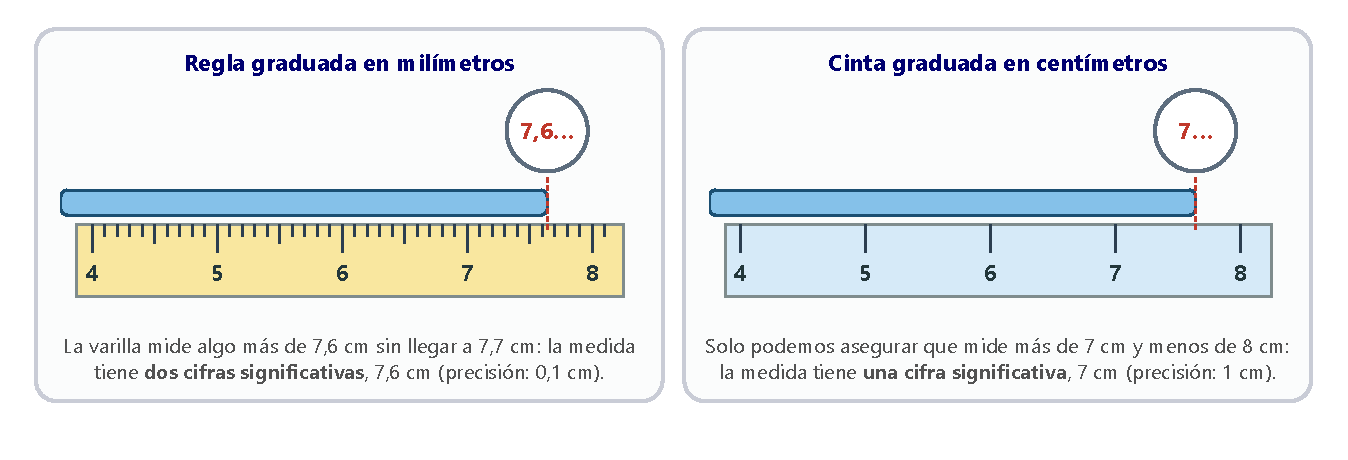
\includegraphics[width=\textwidth]{images/UD1/precision}
    \caption{La misma varilla medida con dos instrumentos de distinta precisión.}
    \label{fig:precision}
\end{figure}

\begin{definition}[Cifras significativas]
    Las \textbf{cifras significativas} de una medida son los dígitos que se conocen con seguridad.
\end{definition}

\begin{itemize}
    \item \textbf{Son significativas} todas las cifras distintas de cero (321 tiene tres; \num{1.345}, cuatro) y los ceros situados entre cifras distintas de cero o detrás de ellas en la parte decimal (\num{106.470} tiene seis).
    \item \textbf{No son significativos} los ceros a la izquierda de la primera cifra distinta de cero (\num{0.405} tiene tres; \num{0.0005090}, cuatro).
\end{itemize}

\subsection{El redondeo}

Al operar con medidas, el resultado no debe tener más cifras significativas que el dato que menos tenga. Se llama \textbf{redondeo} a la eliminación de las cifras situadas a la derecha de la última cifra significativa, con estas reglas:
\begin{itemize}
    \item Si la primera cifra que se elimina es \textbf{mayor que 5} (o un 5 seguido de otras cifras), la anterior aumenta en una unidad: \num{12.56} se redondea a \num{12.6}.
    \item Si es \textbf{menor que 5}, la anterior no cambia: \num{1.43} se redondea a \num{1.4}.
    \item Si es \textbf{exactamente 5}, la anterior aumenta en una unidad si es impar y se deja igual si es par (el cero se considera par): \num{10.35} se redondea a \num{10.4}, y \num{9.25}, a \num{9.2}.
\end{itemize}
Por ejemplo, \(\num{3.5432} + \num{2.531} = \num{6.0742}\), que redondeamos a \num{6.074}; y \(\num{2.33} \cdot \num{2.4} = \num{5.592}\), que redondeamos a \num{5.6}.

\subsection{Los errores en la medida}

Por mucho cuidado que tengamos, el valor medido nunca coincide exactamente con el valor verdadero: \textbf{toda medida está afectada por un error}.
\begin{itemize}
    \item Un \textbf{error accidental} se debe a causas imprevisibles y no aparece siempre (variaciones en las condiciones, apreciación del experimentador\ldots). Puede ser por exceso o por defecto, y se compensa en parte haciendo varias medidas y tomando la \textbf{media}.
    \item Un \textbf{error sistemático} aparece siempre que se mide, porque se debe a un mal funcionamiento del instrumento o al método de medida (por ejemplo, una balanza mal calibrada).
\end{itemize}

\begin{definition}[Error absoluto y error relativo]
    El \textbf{error absoluto}, \(\varepsilon_a\), es la diferencia entre el valor medido, \(x'\), y el valor verdadero, \(x\): \(\varepsilon_a = |x' - x|\). Tiene las mismas unidades que la magnitud.

    El \textbf{error relativo}, \(\varepsilon_r\), es el cociente entre el error absoluto y el valor verdadero: \(\varepsilon_r = \dfrac{\varepsilon_a}{x}\). No tiene unidades y suele expresarse en tanto por ciento. Una medida es más precisa cuanto menor es su error relativo.
\end{definition}

Como no conocemos el valor verdadero, tomamos como tal la \textbf{media} de varias medidas. Una medida no puede tener más cifras que las que indica su error: si medimos una hoja con una regla que aprecia milímetros y obtenemos \qty{28.8}{\cm}, el resultado es \(\num{28.8} \pm \qty{0.1}{\cm}\), no \(\num{28.83} \pm \qty{0.1}{\cm}\).

\begin{marker}
    \textbf{Cómo expresar el resultado de una medida directa:}
    \begin{enumerate}[label=\arabic*.]
        \item Se hacen varias medidas (al menos tres).
        \item Se calcula su media, \(x_\text{media}\), que se toma como valor verdadero.
        \item Se toma como error absoluto la precisión del instrumento.
        \item El resultado es \(x_\text{media} \pm \varepsilon_a\) (con su unidad), y se calcula el error relativo.
    \end{enumerate}
\end{marker}

\begin{example}
    Medimos el grosor de una moneda con un instrumento que aprecia \qty{0.01}{\mm} y obtenemos \qty{1.20}{\mm}, \qty{1.19}{\mm} y \qty{1.21}{\mm}. Expresa el resultado y calcula el error relativo.

    \[ x_\text{media} = \frac{\num{1.20} + \num{1.19} + \num{1.21}}{3} = \qty{1.20}{\mm} \]
    El resultado es \textcolor{red}{\(\num{1.20} \pm \qty{0.01}{\mm}\)}.
    \(\varepsilon_r = \dfrac{\num{0.01}}{\num{1.20}} = \num{8.3e-3} = \textcolor{red}{\qty{0.83}{\percent}}\).
\end{example}

\begin{exercise}
    Indica el número de cifras significativas: a) \qty{1525}{\kelvin}; b) \qty{3.0}{\kg}; c) \qty{0.125}{\ampere}; d) \qty{0.425}{\m}; e) \qty{5.1}{\s}; f) \qty{105.40}{\cm}; g) \qty{20.15}{\mL}; h) \qty{9.27}{\km}.
    \begin{solu}
        a) \textcolor{red}{4}; b) \textcolor{red}{2}; c) \textcolor{red}{3}; d) \textcolor{red}{3}; e) \textcolor{red}{2}; f) \textcolor{red}{5}; g) \textcolor{red}{4}; h) \textcolor{red}{3}.
    \end{solu}
\end{exercise}

\begin{exercise}
    Medimos la temperatura de una disolución con un termómetro cuya precisión es \qty{0.5}{\degreeCelsius}. a) ¿Podemos decir que la temperatura es \(\num{54.4} \pm \qty{0.5}{\degreeCelsius}\)? b) ¿Cómo la expresaríamos correctamente?
    \begin{solu}
        a) \textcolor{red}{No}: con una escala que va de medio en medio grado no podemos leer \num{54.4}; las lecturas posibles son \num{54.0}, \num{54.5}\ldots{} b) Por ejemplo, \textcolor{red}{\(\num{54.5} \pm \qty{0.5}{\degreeCelsius}\)}.
    \end{solu}
\end{exercise}

\begin{exercise}
    Medimos el grosor del lomo de un libro con una regla que aprecia milímetros y obtenemos \qty{19.0}{\mm}. a) ¿Cuál es el error absoluto? Expresa el resultado. b) Calcula el error relativo.
    \begin{solu}
        a) \(\varepsilon_a = \qty{1}{\mm}\); resultado: \textcolor{red}{\(19 \pm \qty{1}{\mm}\)}. b) \(\varepsilon_r = \dfrac{1}{19} \cdot 100 = \textcolor{red}{\qty{5.3}{\percent}}\).
    \end{solu}
\end{exercise}

\subsection*{Actividades de consolidación: la expresión de la medida}

\begin{exercise}
    Asocia cada concepto con su definición. Conceptos: redondeo, cifra significativa, error accidental, error sistemático, error absoluto, error relativo, valor verdadero.
    \begin{enumerate}[label=\alph*)]
        \item Error debido a una causa imprevisible que no se presenta siempre.
        \item Dígito que se conoce con seguridad en una medida.
        \item Error debido al mal funcionamiento del instrumento o al método de medida.
        \item Eliminación de las cifras situadas a la derecha de la última cifra significativa.
        \item En una medida directa, coincide con la precisión del instrumento.
        \item Media de todas las medidas realizadas.
        \item Cociente entre el error absoluto y el valor verdadero.
    \end{enumerate}
    \begin{solu}
        a) \textcolor{red}{Error accidental}; b) \textcolor{red}{cifra significativa}; c) \textcolor{red}{error sistemático}; d) \textcolor{red}{redondeo}; e) \textcolor{red}{error absoluto}; f) \textcolor{red}{valor verdadero}; g) \textcolor{red}{error relativo}.
    \end{solu}
\end{exercise}

\begin{exercise}
    ¿Cuántas cifras significativas tienen estas masas, en kg? a) 543; b) \num{5.622}; c) \num{42.0}; d) \num{105.320}; e) \num{0.05}; f) \num{9.29}.
    \begin{solu}
        a) \textcolor{red}{3}; b) \textcolor{red}{4}; c) \textcolor{red}{3}; d) \textcolor{red}{6}; e) \textcolor{red}{1}; f) \textcolor{red}{3}.
    \end{solu}
\end{exercise}

\begin{exercise}
    Redondea a una cifra decimal (en cm): a) \num{10.68}; b) \num{1.08}; c) \num{2.42}; d) \num{10.55}; e) \num{104.20}; f) \num{9.65}.
    \begin{solu}
        a) \textcolor{red}{\num{10.7}}; b) \textcolor{red}{\num{1.1}}; c) \textcolor{red}{\num{2.4}}; d) \textcolor{red}{\num{10.6}} (el 5 sigue a un 5, impar); e) \textcolor{red}{\num{104.2}}; f) \textcolor{red}{\num{9.6}} (el 5 sigue a un 6, par).
    \end{solu}
\end{exercise}

\begin{exercise}
    Un joyero mide varias veces la masa de una joya: \qty{4.25}{\gram}, \qty{4.28}{\gram}, \qty{4.27}{\gram}, \qty{4.23}{\gram}, \qty{4.26}{\gram}, \qty{4.27}{\gram} y \qty{4.26}{\gram}. a) Expresa el resultado con su error absoluto. b) Calcula el error relativo.
    \begin{solu}
        a) \(x_\text{media} = \dfrac{\num{29.82}}{7} = \qty{4.26}{\gram}\). La balanza aprecia centésimas de gramo, así que \(\varepsilon_a = \qty{0.01}{\gram}\): \textcolor{red}{\(\num{4.26} \pm \qty{0.01}{\gram}\)}.
        b) \(\varepsilon_r = \dfrac{\num{0.01}}{\num{4.26}} \cdot 100 = \textcolor{red}{\qty{0.23}{\percent}}\).
    \end{solu}
\end{exercise}

\begin{exercise}
    Con un péndulo simple determinamos la aceleración de la gravedad y obtenemos (en \unit{\m\per\square\s}): \num{9.82}, \num{9.84}, \num{9.89}, \num{9.79}, \num{9.91}, \num{9.83}. a) Calcula el valor medio y su error absoluto. b) Halla el error relativo.
    \begin{solu}
        a) \(g_\text{media} = \dfrac{\num{59.08}}{6} = \num{9.847} \approx \qty{9.85}{\m\per\square\s}\). Es una medida \emph{indirecta} (\(g\) se calcula a partir de otras medidas), así que no hay precisión de un aparato; tomamos como error la media de las desviaciones respecto al valor medio:
        \(\varepsilon_a = \dfrac{\num{0.03} + \num{0.01} + \num{0.04} + \num{0.06} + \num{0.06} + \num{0.02}}{6} = \num{0.04}\). Resultado: \textcolor{red}{\(\num{9.85} \pm \qty{0.04}{\m\per\square\s}\)}.
        b) \(\varepsilon_r = \dfrac{\num{0.04}}{\num{9.85}} \cdot 100 = \textcolor{red}{\qty{0.4}{\percent}}\).
    \end{solu}
\end{exercise}

\begin{exercise}
    Con una balanza digital que aprecia miligramos obtenemos (en g): \num{18.464}, \num{18.462}, \num{18.465}, \num{18.464}, \num{18.463}, \num{18.463}. a) Expresa el resultado. b) Calcula el error relativo.
    \begin{solu}
        a) \(x_\text{media} = \dfrac{\num{110.781}}{6} = \num{18.4635} \approx \qty{18.464}{\gram}\) (el 5 sigue a un 3, impar). Resultado: \textcolor{red}{\(\num{18.464} \pm \qty{0.001}{\gram}\)}.
        b) \(\varepsilon_r = \dfrac{\num{0.001}}{\num{18.464}} \cdot 100 = \textcolor{red}{\qty{0.0054}{\percent}}\).
    \end{solu}
\end{exercise}

\begin{exercise}
    Medimos la anchura de un móvil con una regla que aprecia milímetros y obtenemos \qty{7.0}{\cm}. a) ¿Cuál es el error absoluto? Expresa el resultado. b) Calcula el error relativo.
    \begin{solu}
        a) \(\varepsilon_a = \qty{0.1}{\cm}\): \textcolor{red}{\(\num{7.0} \pm \qty{0.1}{\cm}\)}. b) \(\varepsilon_r = \dfrac{\num{0.1}}{\num{7.0}} \cdot 100 = \textcolor{red}{\qty{1.4}{\percent}}\).
    \end{solu}
\end{exercise}

%========================================================================================
\section[Magnitudes escalares y vectoriales]{¿En qué se diferencian las magnitudes escalares de las vectoriales?}
%========================================================================================

Si leemos la temperatura en un termómetro, no necesitamos más información. Pero si nos dicen que un coche va a \qty{36}{\km\per\hour}, para saber dónde estará dentro de un rato necesitamos conocer también hacia dónde va.

\begin{definition}[Magnitudes escalares y vectoriales]
    Una \textbf{magnitud escalar} queda especificada completamente con un número y su unidad: la masa, la densidad, la temperatura, el tiempo, la presión, la energía\ldots{} Se opera con ellas siguiendo las reglas de la aritmética.

    Una \textbf{magnitud vectorial} queda definida por su \textbf{módulo} (valor numérico), su \textbf{dirección} (recta sobre la que actúa), su \textbf{sentido} y su \textbf{punto de aplicación}: la velocidad, la aceleración, la fuerza, el desplazamiento\ldots{} Se representan mediante \textbf{vectores}, con una flecha sobre el símbolo: \(\vec{v}\).
\end{definition}

Un \textbf{vector} es un segmento orientado: su longitud representa el módulo, la recta que lo contiene es la dirección, la punta de flecha indica el sentido y su origen es el punto de aplicación (figura~\ref{fig:vectores}). Dos vectores son \textbf{opuestos} si tienen el mismo módulo y la misma dirección, pero sentidos contrarios: \(\vec{a} = -\vec{b}\).

\begin{figure}[H]
    \centering
    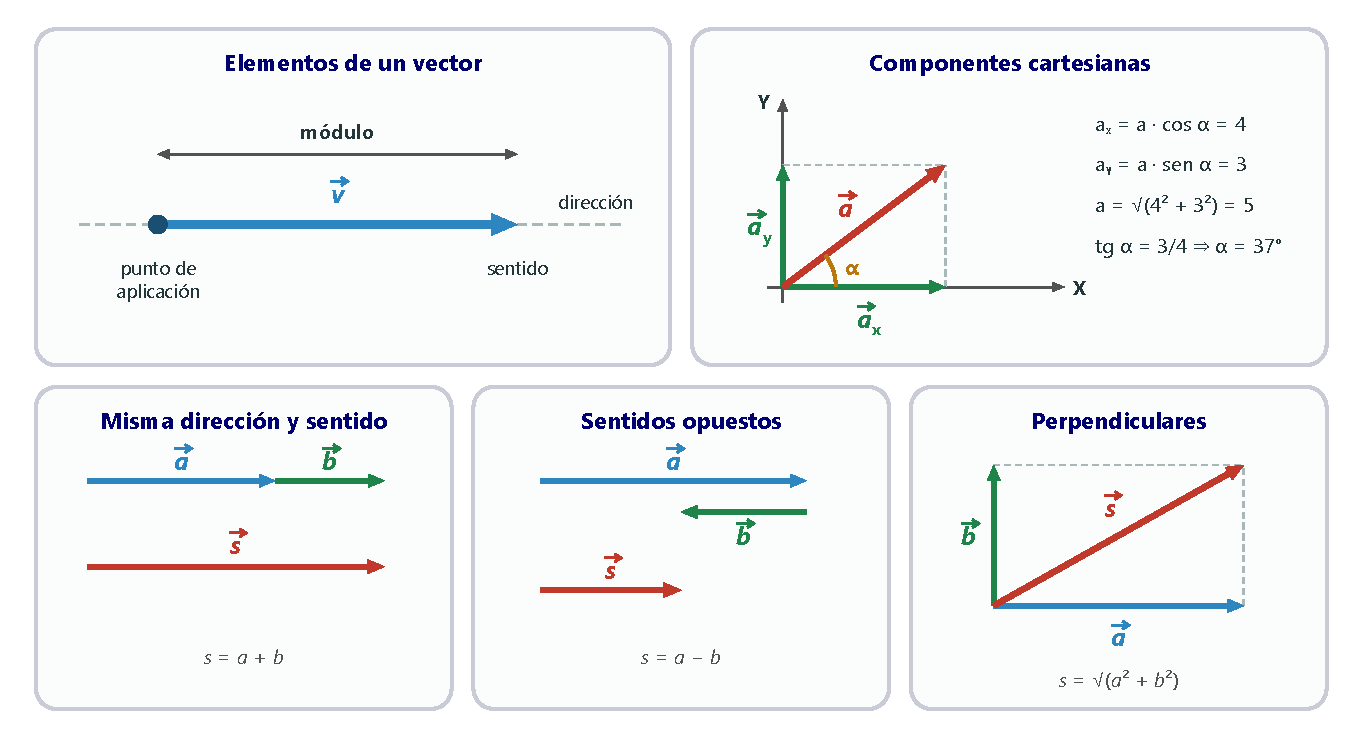
\includegraphics[width=\textwidth]{images/UD1/vectores}
    \caption{Elementos de un vector, componentes cartesianas y suma de vectores.}
    \label{fig:vectores}
\end{figure}

\subsection{¿Cómo se suman los vectores?}

Para sumar dos vectores, se traslada el segundo paralelamente a sí mismo hasta que su origen coincida con el extremo del primero; el vector suma va desde el origen del primero hasta el extremo del segundo. Si los dos vectores tienen el mismo punto de aplicación, la suma es la diagonal del paralelogramo que forman (\textbf{regla del paralelogramo}). Casos particulares (figura~\ref{fig:vectores}):
\begin{itemize}
    \item \textbf{Misma dirección y sentido}: el módulo de la suma es la suma de los módulos, \(s = a + b\), con la misma dirección y sentido.
    \item \textbf{Misma dirección y sentidos opuestos}: el módulo de la suma es la diferencia de los módulos, \(s = a - b\), con el sentido del mayor.
    \item \textbf{Perpendiculares}: por el teorema de Pitágoras, \(s = \sqrt{a^2 + b^2}\).
\end{itemize}

\subsection{¿Cuáles son las componentes de un vector?}

Cualquier vector puede expresarse como la suma de un vector en el eje X y otro en el eje Y, sus \textbf{componentes cartesianas}: \(\vec{a} = \vec{a}_x + \vec{a}_y\). Si \(\alpha\) es el ángulo que forma con el eje X:
\[ a_x = a \cdot \cos\alpha \qquad a_y = a \cdot \sen\alpha \qquad a = \sqrt{a_x^2 + a_y^2} \qquad \tg\alpha = \frac{a_y}{a_x} \]
Por ejemplo, un vector de módulo 5 que forma \ang{37} con el eje X tiene componentes \(a_x = 4\) y \(a_y = 3\).

\begin{exercise}
    Clasifica en escalares y vectoriales: masa, temperatura, velocidad, tiempo, aceleración y fuerza. Escribe dos ejemplos más de cada tipo.
    \begin{solu}
        Escalares: \textcolor{red}{masa, temperatura y tiempo} (otras: energía, volumen). Vectoriales: \textcolor{red}{velocidad, aceleración y fuerza} (otras: desplazamiento, peso).
    \end{solu}
\end{exercise}

\begin{exercise}
    Dibuja un vector con origen en el origen de coordenadas, de módulo 4, dirección la del eje X y sentido hacia las \(x\) positivas. Dibuja después su opuesto.
    \begin{solu}
        \begin{center}
            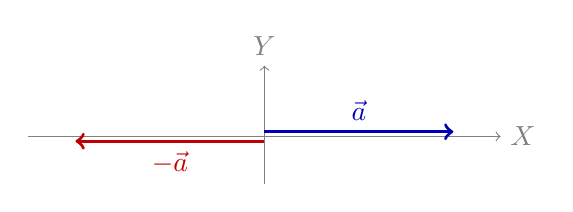
\begin{tikzpicture}[scale=0.6]
                \draw[->, gray] (-5,0) -- (5,0) node[right] {\(X\)}; \draw[->, gray] (0,-1) -- (0,1.5) node[above] {\(Y\)};
                \draw[->, very thick, blue!70!black] (0,0.1) -- (4,0.1) node[above, pos=0.5] {\(\vec{a}\)};
                \draw[->, very thick, red!75!black] (0,-0.1) -- (-4,-0.1) node[below, pos=0.5] {\(-\vec{a}\)};
            \end{tikzpicture}
        \end{center}
        El opuesto tiene el \textcolor{red}{mismo módulo y dirección, pero sentido contrario}.
    \end{solu}
\end{exercise}

\begin{exercise}
    Calcula el módulo de los vectores de componentes: a) \(a_x = 5\), \(a_y = 5\); b) \(b_x = 5\), \(b_y = 7\); c) \(c_x = -5\), \(c_y = -7\). Halla el ángulo que forma cada uno con el eje X.
    \begin{solu}
        a) \(a = \sqrt{25 + 25} = \textcolor{red}{\num{7.07}}\); \(\tg\alpha = 1 \Rightarrow \alpha = \textcolor{red}{\ang{45}}\).
        b) \(b = \sqrt{25 + 49} = \textcolor{red}{\num{8.60}}\); \(\tg\alpha = \num{1.4} \Rightarrow \alpha = \textcolor{red}{\ang{54.5}}\).
        c) \(c = \textcolor{red}{\num{8.60}}\); apunta hacia el tercer cuadrante: \(\alpha = \ang{180} + \ang{54.5} = \textcolor{red}{\ang{234.5}}\).
    \end{solu}
\end{exercise}

\begin{exercise}
    Dibuja dos vectores con el mismo punto de aplicación, direcciones perpendiculares y uno de módulo triple que el otro. Si el menor mide 2, ¿cuánto mide su suma?
    \begin{solu}
        Por ejemplo, \(\vec{a}\) de módulo 2 en el eje X y \(\vec{b}\) de módulo 6 en el eje Y. \(s = \sqrt{2^2 + 6^2} = \textcolor{red}{\num{6.32}}\).
    \end{solu}
\end{exercise}

\subsection*{Actividades de consolidación: magnitudes escalares y vectoriales}

\begin{exercise}
    Clasifica en escalares y vectoriales: presión, volumen, temperatura, masa, densidad, velocidad, aceleración, aceleración de la gravedad, tiempo, desplazamiento, potencia y energía térmica.
    \begin{solu}
        Escalares: \textcolor{red}{presión, volumen, temperatura, masa, densidad, tiempo, potencia y energía térmica}. Vectoriales: \textcolor{red}{velocidad, aceleración, aceleración de la gravedad y desplazamiento}.
    \end{solu}
\end{exercise}

\begin{exercise}
    ¿Qué elementos tiene un vector? ¿Por qué se dice que la fuerza es una magnitud vectorial? Indica si cada descripción corresponde a una magnitud escalar o vectorial: a) hay que especificar su punto de aplicación; b) se cuantifica con un número y su unidad; c) se representa con un vector; d) hay que especificar su dirección y sentido.
    \begin{solu}
        \textcolor{red}{Módulo, dirección, sentido y punto de aplicación}. La fuerza es vectorial porque su efecto depende también de hacia dónde y dónde se aplica. Escalar: \textcolor{red}{b)}; vectorial: \textcolor{red}{a), c) y d)}.
    \end{solu}
\end{exercise}

\begin{exercise}
    Calcula la suma de dos vectores de módulos 7 y 9 aplicados en el mismo punto si: a) tienen la misma dirección y sentido; b) la misma dirección y sentidos opuestos; c) son perpendiculares.
    \begin{solu}
        a) \(7 + 9 = \textcolor{red}{16}\); b) \(9 - 7 = \textcolor{red}{2}\), en el sentido del de módulo 9; c) \(\sqrt{49 + 81} = \textcolor{red}{\num{11.4}}\).
    \end{solu}
\end{exercise}

\begin{exercise}
    Tres vectores están aplicados en el origen: \(\vec{a}\), de módulo 3, apunta hacia las \(x\) positivas; \(\vec{b}\), de módulo 3, hacia las \(x\) negativas; \(\vec{c}\), de módulo 5, hacia las \(y\) negativas. a) ¿Qué vectores tienen la misma dirección? ¿Y el mismo módulo? b) Describe el opuesto de \(\vec{c}\). c) Calcula \(\vec{a} + \vec{b}\) y \(\vec{a} + \vec{c}\).
    \begin{solu}
        a) \(\vec{a}\) y \(\vec{b}\) tienen la \textcolor{red}{misma dirección} (eje X) y el \textcolor{red}{mismo módulo}, pero sentidos opuestos: son opuestos.
        b) \(-\vec{c}\): módulo 5, dirección del eje Y, \textcolor{red}{sentido hacia las \(y\) positivas}.
        c) \(\vec{a} + \vec{b} = \vec{0}\) (módulo \textcolor{red}{0}); \(|\vec{a} + \vec{c}| = \sqrt{9 + 25} = \textcolor{red}{\num{5.83}}\).
    \end{solu}
\end{exercise}

\begin{exercise}
    Los vectores \(\vec{a}\) (módulo 2) y \(\vec{b}\) (módulo 3) apuntan hacia la derecha, y \(\vec{c}\) (módulo 6), hacia la izquierda, todos en la misma dirección. Calcula: a) \(\vec{a} + \vec{b}\); b) \(\vec{a} + \vec{b} + \vec{c}\); c) \(\vec{b} - \vec{a}\).
    \begin{solu}
        a) Módulo \textcolor{red}{5}, hacia la derecha. b) \(5 - 6\): módulo \textcolor{red}{1}, hacia la izquierda. c) Módulo \textcolor{red}{1}, hacia la derecha.
    \end{solu}
\end{exercise}

\begin{exercise}
    a) Calcula la suma de dos vectores perpendiculares de módulo 50 aplicados en el mismo punto. b) La suma de dos vectores perpendiculares vale \num{8.6} y uno mide 5. ¿Cuánto mide el otro? c) ¿Cuánto vale la suma de dos vectores de módulos 3 y 4 si son paralelos del mismo sentido, de sentido opuesto o perpendiculares?
    \begin{solu}
        a) \(\sqrt{50^2 + 50^2} = \textcolor{red}{\num{70.7}}\).
        b) \(\num{8.6}^2 = 5^2 + b^2 \Rightarrow b = \sqrt{\num{73.96} - 25} = \textcolor{red}{7}\).
        c) \textcolor{red}{7}; \textcolor{red}{1}; \(\sqrt{9 + 16} = \textcolor{red}{5}\).
    \end{solu}
\end{exercise}

%========================================================================================
\section[El laboratorio de física y química]{Normas de seguridad en el laboratorio de física y química}
%========================================================================================

Los laboratorios de física y química están preparados para experimentar e investigar. Tienen agua corriente, electricidad y a veces gas, mesas y armarios adecuados, campanas extractoras de gases, extintores, lavaojos y un botiquín. Para evitar accidentes hay que seguir estas normas:

\begin{enumerate}[label=\numberballblue]
    \item Localiza las salidas de emergencia, los extintores, los lavaojos y los equipos de emergencia. No corras dentro del laboratorio.
    \item Mantén el área de trabajo limpia, ordenada y con solo el material que vayas a usar.
    \item Usa bata (abrochada) y guantes; y gafas de seguridad cuando manejes productos tóxicos o corrosivos.
    \item Maneja el material de vidrio con cuidado. Si se rompe, deposítalo en el contenedor para vidrio, nunca en la papelera.
    \item No manipules sustancias inflamables cerca de fuentes de calor. Calienta los tubos de ensayo con pinzas de madera, inclinados y sin apuntar con ellos a nadie.
    \item No toques aparatos eléctricos con las manos mojadas ni los dejes cerca de líquidos.
    \item No comas ni bebas en el laboratorio, y lávate las manos al salir.
    \item Trabaja en la campana extractora con las sustancias o reacciones que desprenden gases.
    \item No viertas residuos por el desagüe, sino en los recipientes destinados a ellos, y no devuelvas los restos de reactivo a los frascos originales.
    \item No pipetees nunca con la boca: usa una pera o un pipeteador. Tapa los frascos después de usarlos.
\end{enumerate}

\begin{figure}[H]
    \centering
    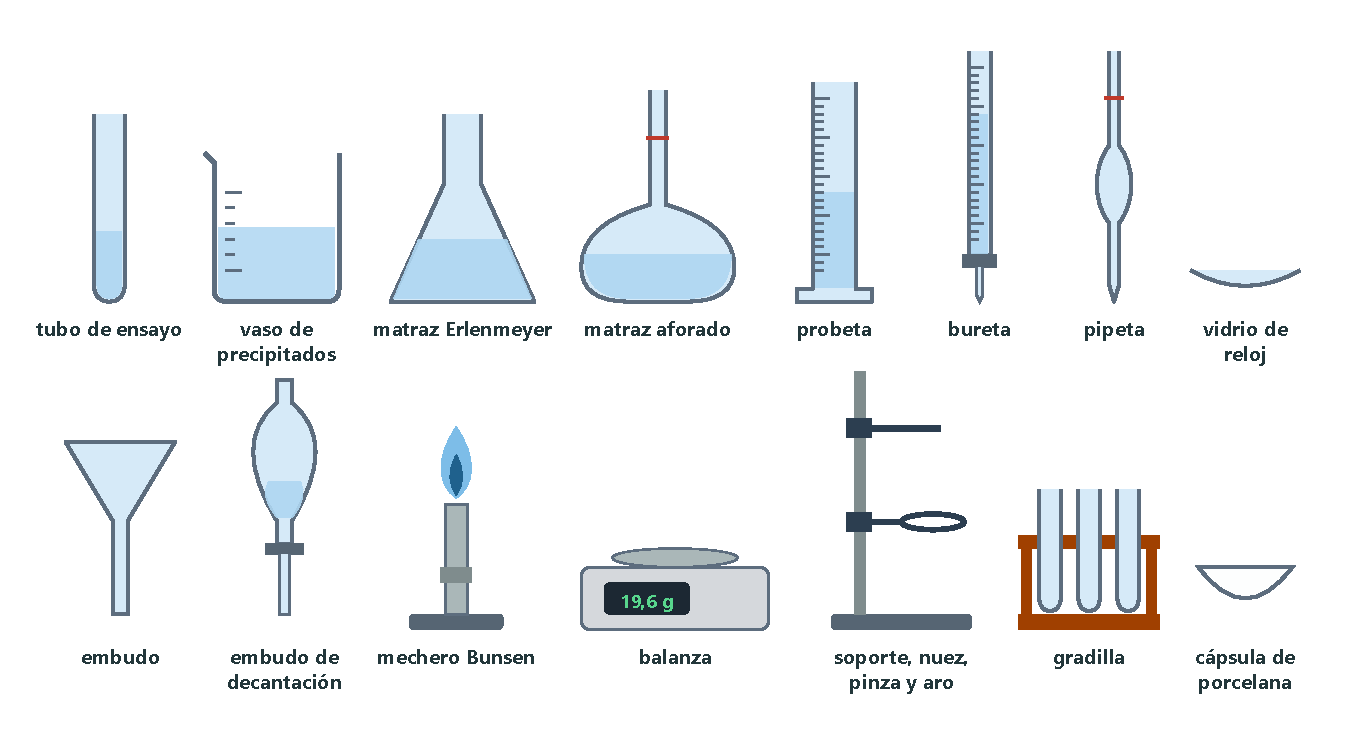
\includegraphics[width=\textwidth]{images/UD1/material_laboratorio}
    \caption{Material de laboratorio de uso frecuente.}
    \label{fig:material_laboratorio}
\end{figure}

Las etiquetas de los productos químicos informan de sus peligros mediante unos \textbf{pictogramas} normalizados: un símbolo negro sobre fondo blanco, dentro de un rombo con borde rojo (figura~\ref{fig:pictogramas}).

\begin{figure}[H]
    \centering
    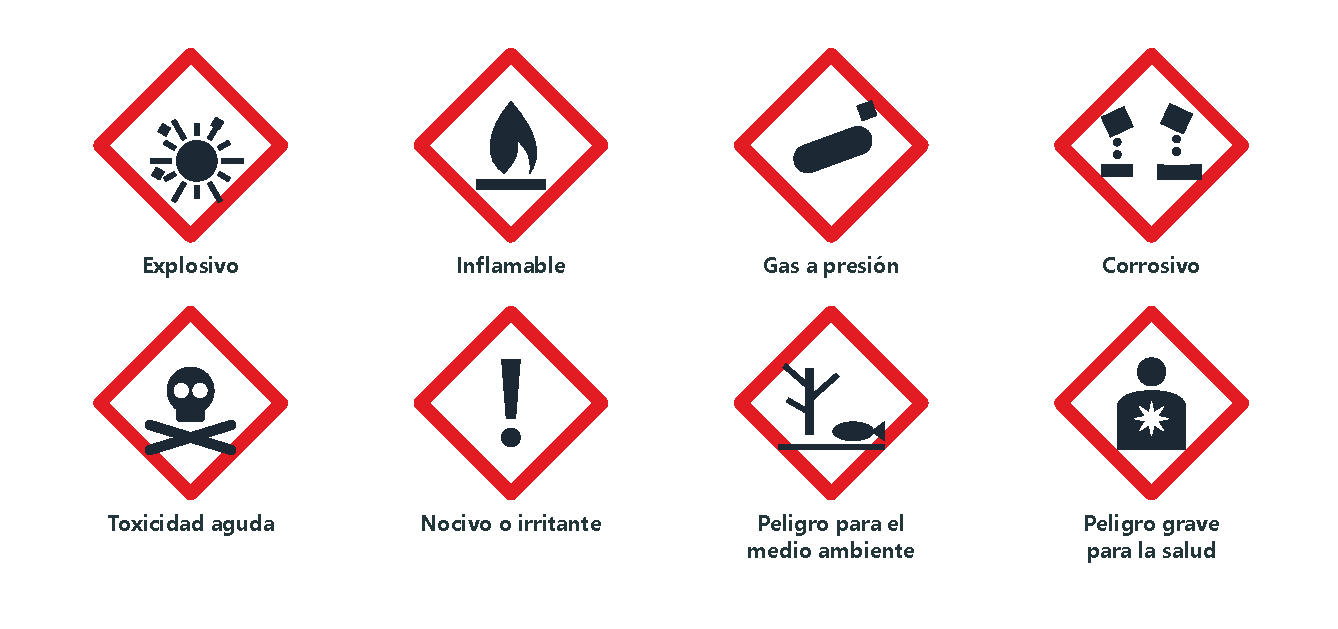
\includegraphics[width=\textwidth]{images/UD1/pictogramas}
    \caption{Pictogramas de peligro de los productos químicos.}
    \label{fig:pictogramas}
\end{figure}

\begin{exercise}
    Busca información sobre los pictogramas de la figura~\ref{fig:pictogramas} y explica qué normas de seguridad reducen el riesgo de cada uno.
    \begin{solu}
        Respuesta abierta. \textcolor{red}{Explosivo}: evitar golpes, fricción y calor. \textcolor{red}{Inflamable}: alejar de llamas y fuentes de calor. \textcolor{red}{Gas a presión}: no calentar las botellas y sujetarlas bien. \textcolor{red}{Corrosivo}: usar guantes y gafas. \textcolor{red}{Toxicidad aguda}: no inhalar, ingerir ni tocar; usar la campana y guantes. \textcolor{red}{Nocivo o irritante}: evitar el contacto con la piel y los ojos. \textcolor{red}{Peligro para el medio ambiente}: no verterlo por el desagüe. \textcolor{red}{Peligro grave para la salud}: protección completa y mínima exposición.
    \end{solu}
\end{exercise}

\begin{exercise}
    Nombra el material de la figura~\ref{fig:material_laboratorio} que usarías para: a) medir un volumen de líquido con precisión; b) preparar \qty{250}{\mL} exactos de una disolución; c) calentar una sustancia; d) separar dos líquidos que no se mezclan; e) medir la masa de un sólido.
    \begin{solu}
        a) Una \textcolor{red}{probeta}, una \textcolor{red}{pipeta} o una \textcolor{red}{bureta}; b) un \textcolor{red}{matraz aforado}; c) un \textcolor{red}{mechero Bunsen} (con un tubo de ensayo o un vaso de precipitados); d) un \textcolor{red}{embudo de decantación}; e) una \textcolor{red}{balanza}.
    \end{solu}
\end{exercise}
